\documentclass{article}
\usepackage[utf8]{inputenc}
\usepackage{graphicx}
\usepackage[margin=0.5in]{geometry}
\usepackage{amsmath}


\title{Inferring mutational fitness costs in HIV from within-patient frequencies}
\author{Marion Hartl\footnote{These authors contributed equally and are listed in alphabetical order} \footnote{Department of Biology, San Francisco State University, San Francisco, California, USA}, Kristof Theys \footnotemark[1] \footnote{Clinical and Epidemiological Virology, Department of Microbiology and Immunology, Rega Institute for Medical Research, KU Leuven - University of Leuven , Leuven, Belgium}, 
Alison Feder \footnote{Department of Biology, Stanford University, Paolo Alto, California, USA}, Maoz Gelbart \footnote{Department of Molecular Microbiology and Biotechnology, George S. Wise Faculty of Life Sciences, Tel Aviv University, Tel Aviv, Israel}, Adi Stern \footnotemark[5], Pleuni S. Pennings \footnotemark[2]}

\date{May 2016}

\begin{document}

\maketitle{}
\section{Abstract}
%150 words for Elife
%PSP: it is too long now, but I think that's OK for the biorxiv.
The human immunodeficiency virus (HIV) has a high mutation rate and 
exhibits remarkable genetic diversity. However, we know little about the fitness cost of mutations as they occur \textit {in vivo}. Here, we developed a new framework to estimate fitness costs of single nucleotide mutations. We analyzed a data set of HIV sequences from 160 patients, and calculated the mean mutation frequency across all patients for each of 870 sites of the \textit{pol} gene. 
This allowed us to determine the differential cost of nonsense, non-synonymous and synonymous mutations. We found that non-synonymous mutations that lead to drastic amino acid changes are three times more costly than those that do not, mutations that create new CpG dinucleotides are up to four times more costly than those that do not, and G $\rightarrow$ A mutations are more than twice as costly as A $\rightarrow$ G mutations. Finally, we discovered that  within-patient mutation frequencies are highly correlated with substitution frequencies across the global HIV pandemic. We anticipate that this new approach will provide insights into the fitness landscape and evolvability of not only HIV, but a variety of viruses and other microbes. 

%What about this for the elife abstract? (149 words)
%HIV has a high mutation rate and exhibits remarkable genetic diversity. However, we know little about the fitness cost of HIV mutations \textit {in vivo}. We calculated the mean frequency of mutations at 870 sites of the \textit{pol} gene gene in 160 patients, allowing us to determine the differential cost of different types of mutations. We found that non-synonymous mutations that lead to drastic amino acid changes are three times more costly than those that do not, mutations that create new CpG dinucleotides are up to four times more costly than those that do not, and G $\rightarrow$ A mutations are more than twice as costly as A $\rightarrow$ G mutations. In addition, within-patient mutation frequencies are highly correlated with substitution frequencies across the global HIV pandemic. We anticipate our new approach will provide insights into the fitness landscape and evolvability of not only HIV, but a variety of microbes.

\section{Introduction}
The human immunodeficiency virus (HIV) replicates with an extremely high mutation rate and exhibits significant genetic diversity within an infected host, often referred to as a "mutant cloud" or "quasispecies" \cite{batschelet1976proportion,domingo1978nucleotide, eigen1993viral,rouzine2001transition, wilke2005quasispecies, biebricher2006quasispecies,lauring2010quasispecies}. Although mutations are crucial for all adaptive processes, they are also associated with fitness costs.   
Thus, to understand the evolution of HIV, it is important to know the fitness costs of mutations \textit {in vivo}. Fitness costs influence the probability of evolution from standing genetic variation (often referred to as pre-existing mutations). Fitness costs also determine the effects of background selection (i.e., the effects of linked deleterious mutations on neutral or beneficial mutations) and thus affect optimal recombination rates. 
All of these processes affect drug resistance and immune escape in HIV \cite{pennings2012standing, Paredes:2010aa, li2011low, neher2010recombination, batorsky2011estimate}. % PSP I changed this back to original text, because causal relationship wasn't correct in new sentence. 
In addition to a better understanding of evolutionary processes in HIV and in general, a detailed knowledge of costs of mutations can also help us to discover new functional elements in the HIV genome.

%I think I like this paragraph better without the first sentence. What do you think?
Costly mutations, which are also referred to as deleterious mutations, are purged from a population by selection \cite{hartl1997principles, trottermutation}. In infinitely large populations, mutations are present at a constant frequency equal to $u/s$, where $u$ is the mutation rate from wild-type to the mutant and $s$ is the selection coefficient that reflects the negative fitness effect or the cost of the mutation. In natural populations of finite size, however, the frequency of mutations is not constant; instead it fluctuates around the expected frequency of $u/s$, because of the stochastic nature of mutation and replication \cite{hartl1997principles}. Due to these stochastic fluctuations, it is impossible to accurately infer the strength of selection acting on individual mutations (i.e., the cost of mutations) from a single observation of a single population.Thus, fitness effects are traditionally assessed either in \textit {in vitro} systems (e.g., cell culture/competition experiments \cite{sanjuan2004distribution, acevedo2014mutational,thyagarajan2014inherent}) or in a phylogenetic framework \cite{lawrie2014comparative,eyre2007distribution,mayrose2013synonymous}. 
% What would you think about adding a sentence or two here stating the limitations of these systems, so readers understand the need for a new approach?
%PSP Yes, good idea. 

HIV has unique properties that allow us to study fitness effects \textit {in vivo}: It is fast evolving \cite{roberts1988accuracy, mansky1995lower, abram2010nature,cuevas2015extremely,zanini2016vivo} and leads to persistent infections \cite{coffin1995hiv,coffin1997retrotransposons, douek2003t}. This means that genetic diversity accumulates quickly and independently in every host, and samples from different patients can thus be treated as independent replicate populations \cite{pennings2014loss}. With data from many replicate populations, the mean frequency of mutations will approach $u/s$ and can be used to estimate their fitness costs, as the fluctuations in mutation frequencies form %represent? 
an ergodic process \cite{karlin2014}. Based on this logic, in this article we present a novel approach that uses observed mutation frequencies in HIV-infected patients to determine the fitness effects of mutations \textit {in vivo}. 

Theoretically, with sufficient sequencing data from enough patient samples, we can use this approach to estimate the \textit {in vivo} fitness cost of every point mutation at every position in the HIV-1 genome. In the current study, we demonstrate its utility by focusing on transition mutations (A$\leftrightarrow$G and C$\leftrightarrow$T) in the first 984 sites of the \textit {pol} gene, which encodes the protease protein and part of the the reverse transcriptase protein, in 160 patients infected with HIV-1 subtype B. We selected transitions because they are much more common in HIV than transversions \cite{abram2010nature}, and thus sufficient data are available to analyze; we selected the \textit {pol} gene because it is highly conserved gene and its products do not come into contact with the immune system \cite{coffin1995hiv, coffin1997retrotransposons}. Finally, we excluded all drug resistance-related sites. Accordingly, most mutations are expected to be deleterious. We report that this test of our method allowed us to quantify many known properties of mutational fitness costs, and also revealed novel insights into the evolutionary constraints of the HIV genome. %Wording OK? I didn't want to go into too much detail in the Intro, since you are about to launch into the Results. But I do want the reader to get a sense of the importance of your findings. You may want to tinker!

%Our analysis is based on observed mutation frequencies in 160 patients who are infected with HIV-1 subtype B, with a median of 19 sequences (range: 2-69) per patient for 984 sites in the \textit {pol} gene \cite{bacheler2000human}, after minimal filtering of the data (see Materials and Methods). First, we find that there is a very clear separation of observed frequencies of synonymous mutations, non-synonymous mutations and nonsense mutations (i.e., mutations that create premature stop codons). Second, we find that inferred costs of mutations are strongly affected by whether the resulting amino-acid change is drastic or not, i.e., costs are lower if a mutation leads to a change to a similar amino acid. Third, we find that mutations that create new CpG sites are more costly than mutations that do not. This finding may reflect selection against CpG sites because they trigger recognition by antiviral defense mechanisms \cite{burns2009genetic, atkinson2014influence, cheng2013cpg}. Fourth, we find that there is a difference in fitness cost depending on which of the four nucleotides is changed, most clearly, G$\rightarrow$A mutations tend to be more costly than the other mutations. Thus, despite the fact we have analysed only a small part of the HIV genome using a dataset with very limited sequencing depth, we succeeded in recovering and quantifying many known properties of mutational fitness costs, combined with novel findings. Our data also allow us to estimate parameters of the entire distribution of fitness effects (DFEs), which may be useful for studies of background selection. Finally, we find that  within-patient frequencies and global frequencies in the subtype B clade are very similar (Pearson's product-moment correlation 0.95), we discuss the possible reasons for this in the discussion.  
%Adi: I think this should move to the discussion: 
%PSP: that's fine with me, not sure where in the discussion though.
%KH: What about the first paragraph of the Discussion? This is a great summary of the key findings.

% Would it be possible to move this to the Discussion as well? 
% Note that in parallel to our study, another study was done that also used HIV within-patient mutation frequencies to estimate fitness costs of mutations \cite{zanini2016vivo}. 

\section{Results}

\subsubsection*{Mean frequency of non-synonymous mutations is lower than that of synonymous mutations}
We began by examining the frequency of the three main categories of mutations: synonymous, non-synonymous and nonsense mutations.  
Since we only considered transitions, there was exactly one possible mutation per site. The \textit {pol} sequence is 984 nucleotides long, but we excluded 75 drug resistance-related sites and 39 protease sites that overlap with Gag, leaving 287 synonymous, 555 non-synonymous and 28 nonsense mutations, for a total of 870 sites. 
For each mutation, we determined the 160 observed frequencies (one for each patient; fewer if a site was filtered out for certain patients, see Material and Methods). 

As an example, we show the frequency spectra at codon 58 of the protease protein, which comprises nucleotides 172 through 174 (Fig.\ref{orderedBacheler}). A transition mutation at the first position (172) creates a premature stop codon. This mutation was never observed in the data and thus has a frequency of zero. A transition mutation at the second codon position (173) leads to an amino acid change (glutamine to arginine) and was found at low frequency. A mutation at the third position of the codon (174) does not change the amino acid and was observed at higher frequency, on average, than the other two mutations (Fig.\ref{orderedBacheler}A).  

We next ordered all sites according to observed mutation frequencies, which revealed that this pattern--synonymous mutations being more common than non-synonymous mutations, which were more common than nonsense mutations--was evident throughout the entire data set. The distributions of the mean frequencies for each of the three main categories of mutations were significantly different (Kolmogorov-Smirnov test, p-value $<$ 2.2e-16 for nonsense vs. non-synonymous sites and for non-synonymous vs. synonymous sites; Fig. \ref{orderedBacheler}B. Nonsense mutations had a frequency of zero, and so did a few non-synonymous mutations. Most non-synonymous mutations had a lower frequency (80\% were present at a frequency lower than 0.01) than synonymous mutations (82\% were present at a frequency higher than 0.01). This difference in distributions probably reflects the higher cost of non-synonymous mutations, which are more likely to directly affect virus replication. 
%KT may 2016; we could make density plots of the two distribution, this can clearly the differences in frequency distributions
%Although a non-synonymous mutation can change the amino acid composition of a protein, synonymous mutations do not affect the amino acid identity. However, there are reported cases in which synonymous mutations change the secondary structure of RNA and thereby affect the stability of the RNA molecule and/or the rate of replication \cite{cuevas2011fitness,martrus2013changes}.
This analysis therefore provides a proof of principle that this approach works: The observed frequencies reflect the relative costs we would expect for these broad categories of mutation.  
%Our analysis of two additional data sets revealed similar results, and can be found in supplementary figures \ref{orderedLehman} and \ref{orderedZanini}.

\begin{figure}[ht!]
\centering
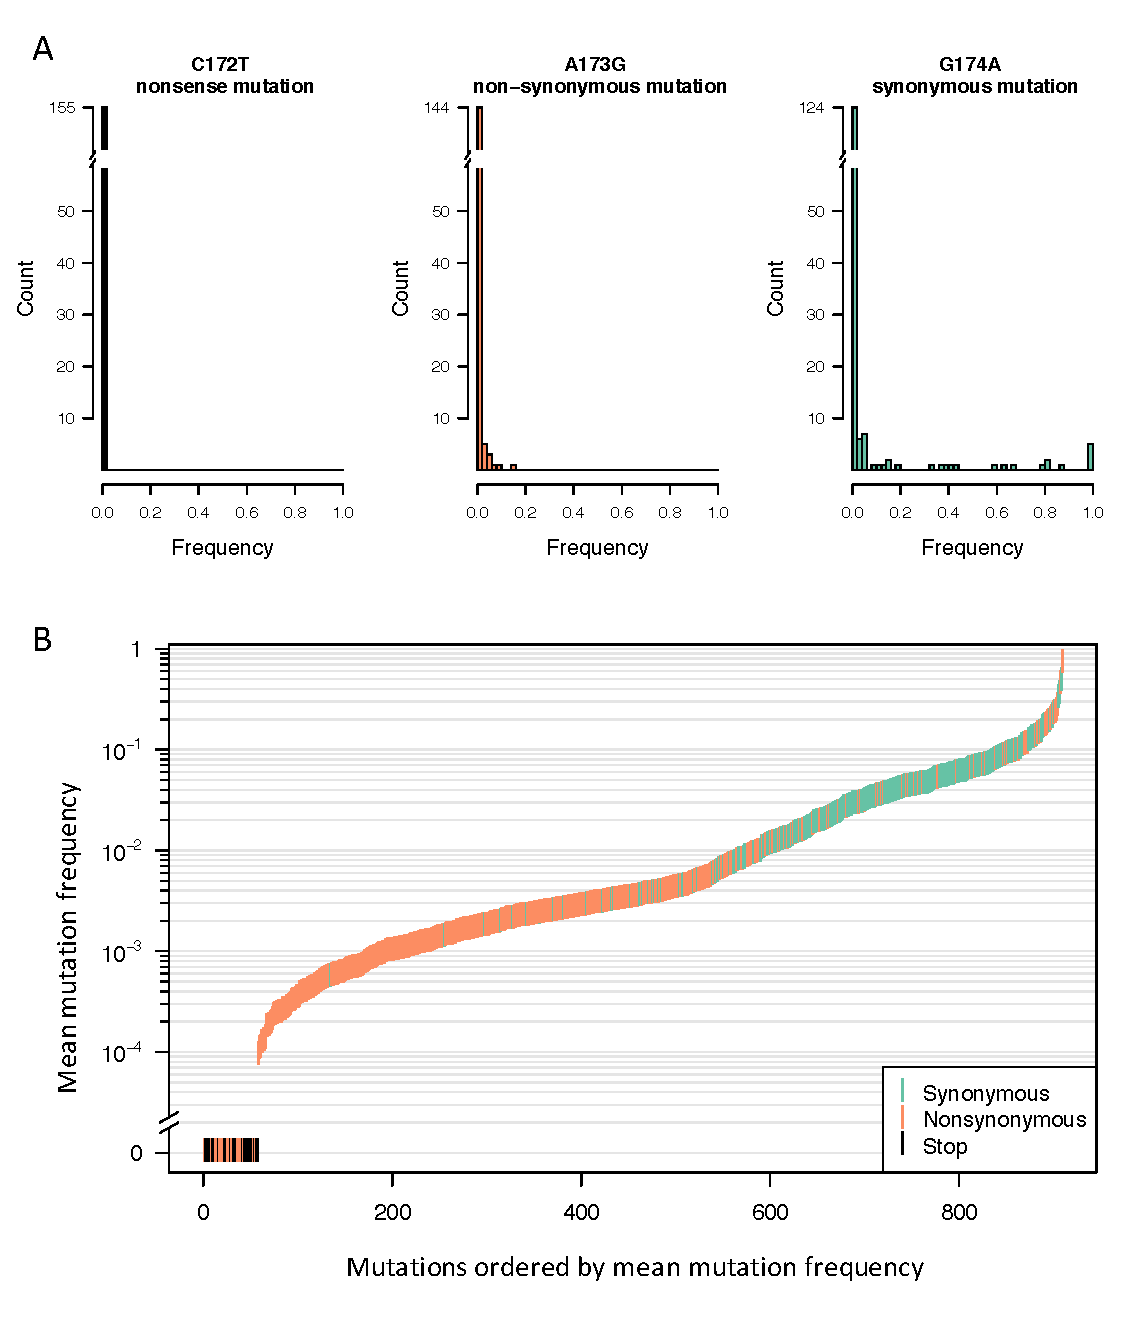
\includegraphics[scale = .8]{F1-grouped.pdf}
%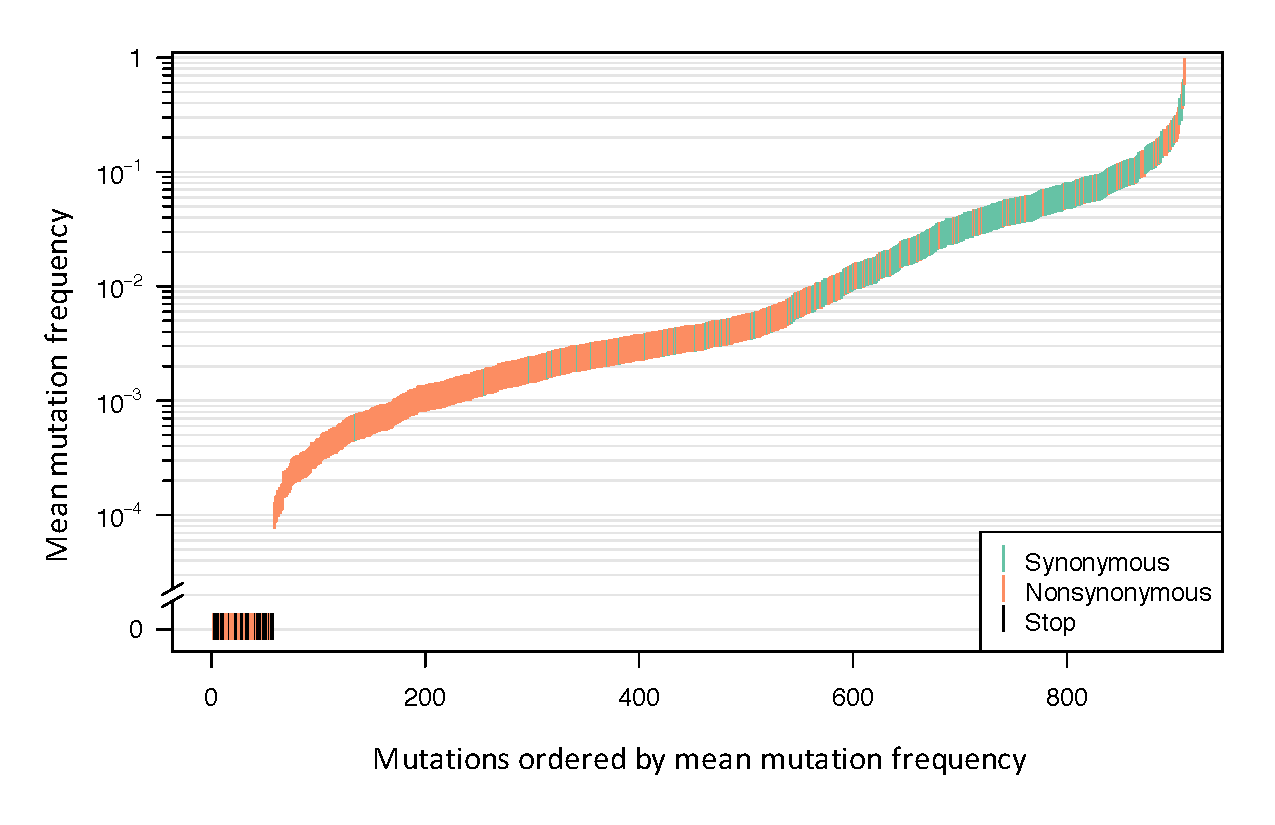
\includegraphics[scale = .8]{Fig1_ordered_Bacheler_cex15.pdf}
% ADI: I think boxplots here for each site, grouped into one figire, would  be more concise... Also the labels at the top can indicate Protease A172G (stop) to give more info on the mutation (for example).
% Another comment: we keep referring over and over to the Bacheler data set. The way I see it, this is the default dataset we report so no need to explicitly refer. When we compare to the others we should refer to them.
%KH: One thing that I like to do in Figure Captions is (when possible) title the figure with a declarative statement about what you want the reader to take away. I think it helps orient the reader to the data. If you like this approach, you might write: "As expected, in the HIV \textit {pol} gene, synonymous mutations occur more frequently than non-synonymous mutations, which occur more frequently than nonsense mutations, which were not observed at all."
\caption{A) The distribution of mutation frequencies plotted for three nucleotide sites in the HIV protease protein (site 172 = nonsense mutation,  site 173 = non-synonymous mutation, site 174 = synonymous mutation). B) Mean mutation frequencies for all sites, ordered by mutation frequency. 
%Since your key contains this information, I would leave the following sentence out.
Nonsense mutations are shown in black, mutations that cause an amino-acid change (non-synonymous) are shown in red and mutations that do not change the amino-acid (synonymous) are shown in green.}
\label{orderedBacheler}
\end{figure}
%PSP: the ordered frequencies figure can't be read when i print it on my black and white printer. should we change the colors?
% Adi: Red and green are also problematic for color-blind. Maybe red and blue would be better.
%I was going to say the same thing! These types of figures are really tough to do well in black and white. 
%\pagebreak

\subsubsection*{Type of amino-acid change and whether a mutation creates a CpG site have major effect on fitness cost}
% use cost (selection coefficent) and then cost only
% are we changing the figure label to " selection coefficient (cost) " as well?
% do not write synonymous sites but syn mutations
% use patient instead of host 
Next, we used a generalized linear model (GLM) to determine the ensemble  characteristics that explain the observed frequencies of synonymous and non-synonymous mutations (see Table \ref{GLM_results}).
%I'm wondering if it would be helpful to the reader to add just a few words to this sentence to make it clear why this alternative approach was used. What was the value added, over and above the approach described in the previous section?
We then used estimated mutation rates from Abram \textit {et al} \cite{abram2010nature}
%,zanini2016population} PSP: I removed the Zanini ref here, we probably should add it when we describe the gamma results. 
and the mutation-selection formula ($f = u / s$) to translate observed frequencies into selection coefficients (costs). 
The estimated costs are shown for some groups of mutations in Figure \ref{modeled_sels}.
As in our first result, overall, synonymous mutations were found at higher frequencies than non-synonymous mutations ($p < 0.0001$), which means that they are less costly.

%synonymous sites first
%can we add a sub-sub-heading for synonymous sites, since the  non-synonymous discussion encompasses multiple paragraphs?
We next sought to determine the characteristics responsible for differences in frequencies, and thus fitness costs, among different synonymous mutations. 
Interestingly, the strongest effect was associated with whether or not a mutation creates a new CpG dinucleotide site (see Table \ref{GLM_results}). 
Specifically, A $\rightarrow$ G mutations and T $\rightarrow$ C mutations that created new CpG sites were found at significantly lower frequencies than A $\rightarrow$ G mutations and T $\rightarrow$ C mutations that did not ($p < 0.0001$). The model predictions for the frequencies suggest that CpG-creating synonymous mutations are four times more costly (selection coefficient appr. $0.001$) than mutations that do not create CpG sites (selection coefficient ~$0.00025$). This finding is consistent with the hypothesis that CpG sites are costly for RNA viruses because they trigger the antiviral cellular response \cite{burns2009genetic, atkinson2014influence}. 
In addition to the strong CpG-creating effect, synonymous G $\rightarrow$ A mutations were found at a frequency lower than expected given their mutation rate. We cannot formally test whether this effect is significant in the GLM framework, but a one-sided, two-sample Wilcoxon test for this comparison showed that the difference in estimated selection coefficients for G $\rightarrow$ A mutations and A $\rightarrow$ G mutations %correct? I wasn't sure about the comparison and filled in with the info below
was highly significant ($p < 0.0001$).
Indeed, the estimated selection coefficients based on the model predictions for the frequencies suggested that synonymous G $\rightarrow$ A mutations are two-and-a-half times as costly as A $\rightarrow$ G mutations ($0.0007$ vs $0.00025$) (Fig. \ref{modeled_sels}). 

%non-synonymous sites
%can we add a sub-sub-heading for non-synonymous sites, since this discussion encompasses multiple paragraphs?
We proceeded to analyze the characteristics associated with frequency differences, and hence fitness costs, in non-synonymous mutations. Here, we distinguished between mutations that led to a drastic amino acid (AA) change and mutations that did not. This distinction was based on the classical grouping of AAs into five groups (positively charged, negatively charged, uncharged, hydrophobic and special cases: cysteine, selenocysteine, glycine and proline); 
%PSP: I added Selenocysteine to this list, as we have it in the methods. 
we defined a change in group as a drastic change. 
Mutations leading to a drastic AA change were found at lower frequency than mutations that did not ($p < 0.0001$). The difference in frequencies suggested a three-fold difference in costs. 
There was also an effect of whether or not non-synonymous mutations led to a CpG site ($p < 0.0001$ for both A $\rightarrow$ G and T $\rightarrow$ C mutations). The difference in frequencies suggests that among mutations that do not lead to a drastic AA change, A $\rightarrow$ G mutations that create a CpG site are about one-and-a-half times more costly than those that do not; similarly, for T $\rightarrow$ C mutations that do not involve a drastic AA change, CpG-forming mutations are three-and-a-half times more costly. In addition, C $\rightarrow$ T and G $\rightarrow$ A mutations appear to be more costly than A $\rightarrow$ G and T $\rightarrow$ C mutations (Fig. \ref{modeled_sels}). We cannot use the GLM framework to test whether this difference is significant, but one-sided two-sample Wilcoxon tests show that the difference in estimated selection coefficients is highly significant ($p < 0.0001$ for both C $\rightarrow$ T and G $\rightarrow$ A mutations when compared with A $\rightarrow$ G mutations). Using model-predicted frequencies and known mutation rates, we estimated that, among non-synonymous mutations that do not involve a drastic AA change or create a CpG site, %OK?
C $\rightarrow$ T mutations are six times more costly than A $\rightarrow$ G mutations, and G $\rightarrow$ A mutations are three-and-a-half times more costly.
% Adi - I'm confused by the below: was the above only for Protease??
%No for both
%Or is this a comparison between Protease and RT? This has to be clarified.... And the SHAPE results??
%Alison tested in her model whether it had an effect to be in RT. That's what I tried to describe in paragraph below.
When we stratified sites by the protein encoded, non-synonymous %correct? this paragraph is all about non-synonymous only, right?
mutations in the reverse transcriptase (RT) portion of the gene had slightly lower frequencies than those in the protease portion ($p < 0.0001$), suggesting that RT mutations are somewhat more costly. Finally, we found a small but significant effect of the SHAPE parameter ($p < 0.0001$), an experimentally determined measure of RNA secondary structure \cite{watts2009architecture}. Specifically, sites with a lower SHAPE parameter (i.e., those more likely to be part of an RNA structure) were associated with lower frequencies (which suggests higher mutational costs), presumably because the secondary structure of the RNA molecule plays a functional role in HIV replication \cite{watts2009architecture} (see Table \ref{GLM_results}). 

%In summary, factors that confer the highest fitness costs to non-synonymous sites were a change of the amino acid group, the creation of a CpG site
%and the ancestral nucleotide. 
%In addition, non-synonymous mutations from C $\rightarrow$ T and G $\rightarrow$ A were in our model more costly than mutating from A $\rightarrow$ G and T $\rightarrow$ C, although this potentially resulted in CpG sites (Figure  \ref{F2}).
Because the nature of the AA change and the ancestral nucleotide
%this is the first time the term "ancestral nucleotide" is being used. Can you explain what you mean by it? I wasn't sure which previous findings involved ancestral nucleotides, so readers might also be confused.
both had a strong effect on costs, we decided to look into this effect more closely. We found that many very costly mutations were associated with a small number of AA changes, starting from glutamate, glycine and proline. This is consistent with our knowledge of protein structures: glycine and proline are often unique and non-replaceable, as the only cyclic and smallest amino acid, respectively. Figure \ref{AA_effect} shows the cost of non-synonymous changes ordered by ancestral and mutant amino acid. These AA effects may be in part responsible for the nucleotide effect we found. %Can you specify which nucleotide effect you are referring to here? 

\begin{figure}[ht!]
\centering
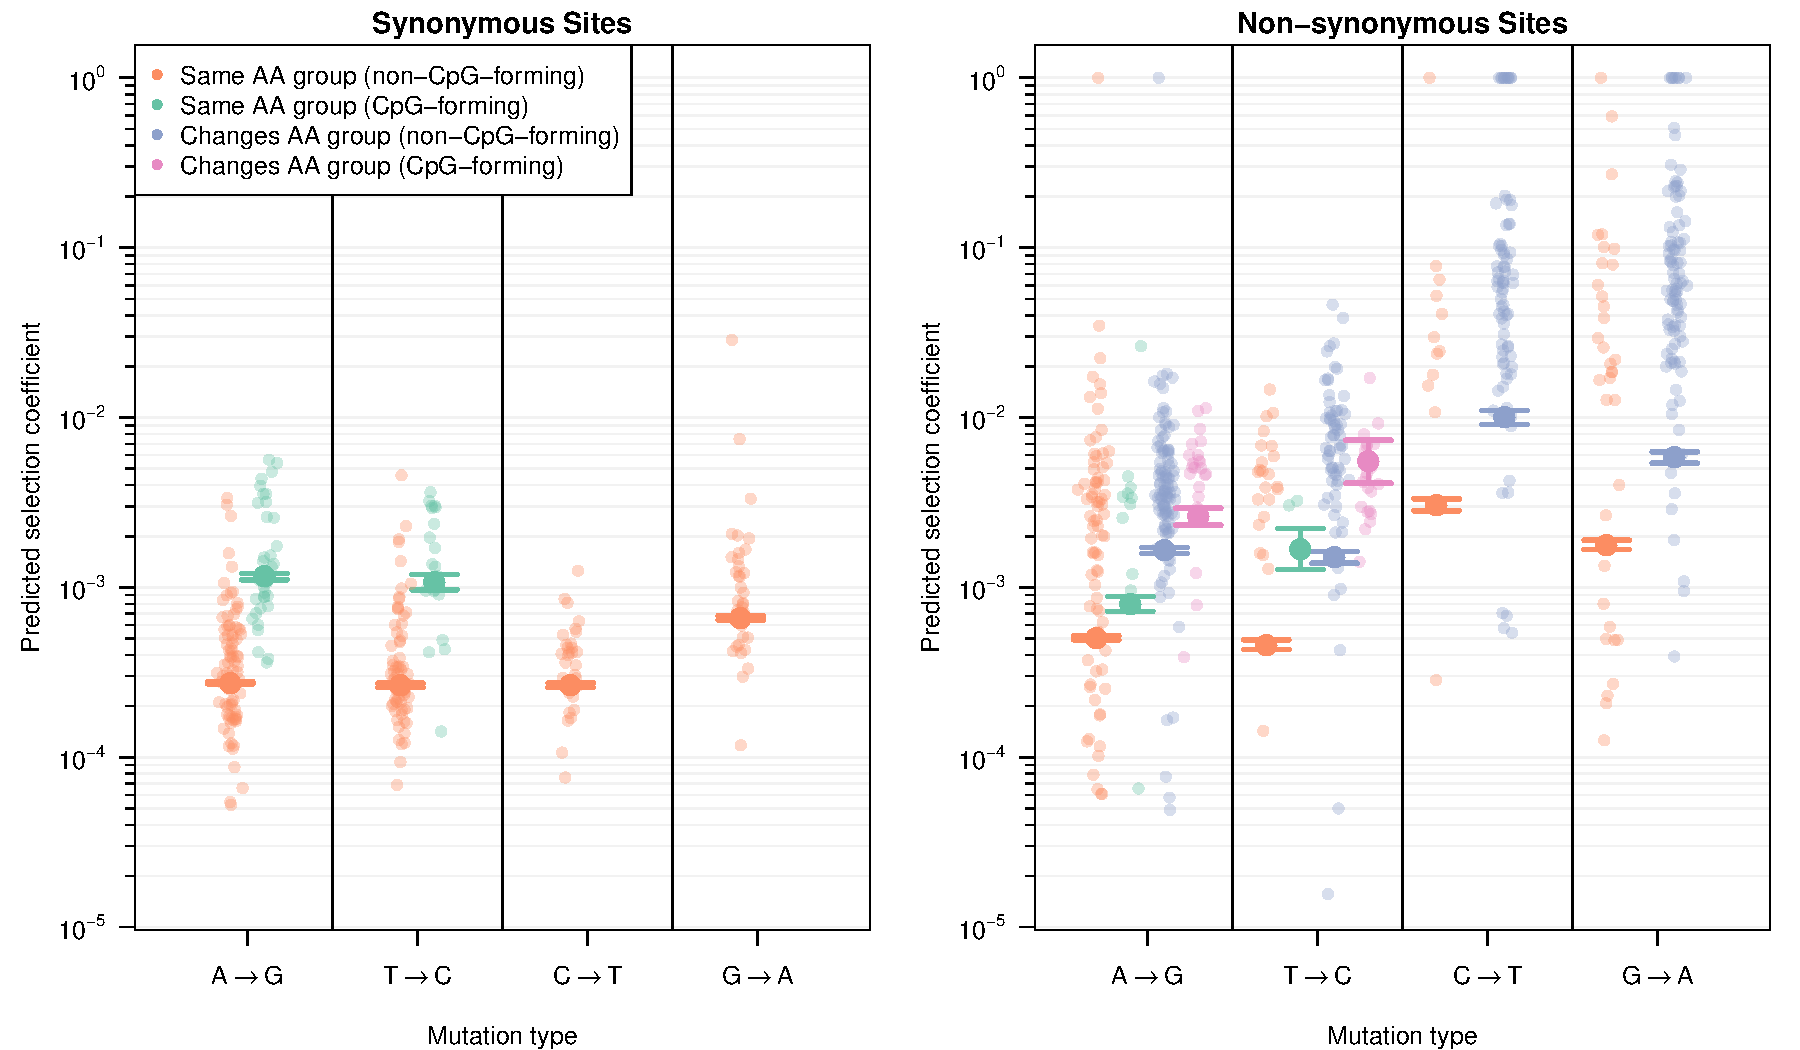
\includegraphics[scale = .6]{F2-modeled_sels.pdf}
\caption{Selection coefficients for transitions at every nucleotide site in the \textit {pol} sequence, estimated using a generalized linear model (GLM) and sequence data from 160 HIV-infected patients, show that CpG site-forming mutations are more costly than non-CpG site-forming mutations and mutations that involve a drastic amino acid change are more costly than mutations that do not.
Shown are predicted selection coefficients for synonymous (\textit {left}) and non-synonymous (\textit {right}) mutations that do not involve a drastic amino acid change and either form CpG sites (\textit {green}) or do not (\textit {orange}). For non-synonymous mutations, predictions are also shown for mutations that do involve drastic amino acid changes and either form CpG sites (\textit {pink}) or do not (\textit {blue"). 
%The cloud of dots in each panel represents the estimated selection coefficients found in the data set.}
%KH: I think readers will assume the former without being told, right?
\label{modeled_sels}
\end{figure}
%KH: What do you think about using the terminology "drastic AA change" instead of "same AA group" in the key? That way it matches the terms that were initially introduced in the text.

% The table below has to include more meaningful names, for example replace t:nonsyn with Non-syn T->C, replace CpG with CpG forming, etc. Why are we including t:CpG if it is not significant?
%KH: Agree, labels need to be more descriptive. Also, I think most journals ask you to replace P=0.000 with <0.001. OK to change in last column?

\begin{table}[ht!]
\centering
\begin{tabular}{lrrrr}
  \hline
 & Estimate & Std. Error & z value & Pr($>$$|$z$|$) \\
 \hline
(Intercept) & -3.208 & 0.013 & -244.671 & 0.000 \\ 
 inRT & 0.136 & 0.008 & 16.206 & 0.000 \\ 
  shape & 0.169 & 0.014 & 12.034 & 0.000 \\ 
  \hline
  t & 0.034 & 0.014 & 2.422 & 0.015 \\ 
  c & 0.808 & 0.016 & 50.379 & 0.000 \\ 
  g & 0.717 & 0.014 & 49.936 & 0.000 \\ 
   CpG & -1.439 & 0.029 & -49.853 & 0.000 \\ 
   t:CpG & 0.041 & 0.047 & 0.875 & 0.381 \\ 
   \hline
  nonsyn & -0.611 & 0.014 & -42.644 & 0.000 \\ 
  t:nonsyn & 0.061 & 0.024 & 2.551 & 0.011 \\ 
  c:nonsyn & -1.833 & 0.037 & -49.396 & 0.000 \\ 
  g:nonsyn & -0.380 & 0.021 & -18.065 & 0.000 \\ 
  nonsyn:CpG & 0.981 & 0.045 & 21.991 & 0.000 \\ 
  t:nonsyn:CpG & -0.881 & 0.093 & -9.447 & 0.000 \\ 
  bigAAChange & -1.183 & 0.014 & -83.501 & 0.000 \\ 
  \hline
\end{tabular}
\caption{Table with GLM results for observed counts of mutants. Significant predictors are listed together with their associated P-value based on a Z-test.}
\label{GLM_results}
\end{table}

 
\pagebreak

\begin{figure}[ht!]
\centering
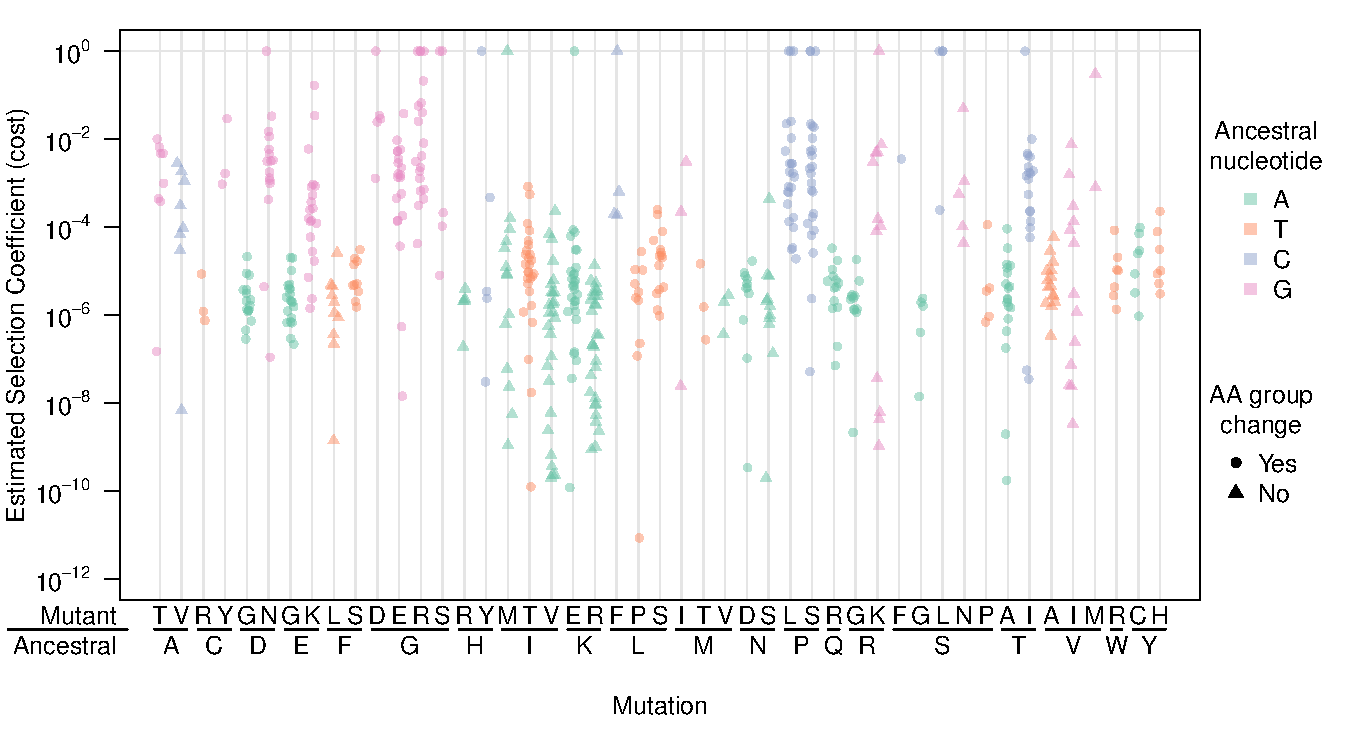
\includegraphics[scale = .7]{aachangesNS.pdf}
\caption{Estimated costs of non-synonymous mutations in the \textit {pol} sequence, ordered by ancestral and mutant amino acid. Colors indicate the different nucleotides, shapes indicate whether the amino acid change is drastic or not.}
\label{AA_effect}
\end{figure}

\subsubsection*{Parameters for gamma distribution of fitness effects}
In addition to the characteristics that determine fitness costs of mutations, we investigated the distribution of fitness effects (DFE). This distribution is of great interest to the evolutionary biology community because it affects standing genetic variation, background selection, and optimal recombination rates \cite{eyre2007distribution}. Moreover, it determines the evolvability of a population: A DFE weighted toward neutral and adaptive mutations reflects a population with more capacity to evolve. Despite their reputation as fast-evolving entities, many viruses have a DFE composed mainly of deleterious and lethal mutations. 
To determine the DFE of HIV, we took the average mutant frequency for each \textit {pol} site and used it to directly estimate the fitness cost using the  mutation-selection formula ($f = u / s$). 
In Figure \ref{Bachelernonsyn}, we show the distributions for each of the ancestral nucleotides, both for synonymous mutations and for non-synonymous mutations (including nonsense mutations). Note that the scales of the x and y-axis differ between the figures. 
We also estimated parameters for the \textit {gamma} distribution that best describes the entire DFE 
%for the part of the \textit {pol} gene that is covered by our data 
(Table \ref{TableGamma}). 

%PSP: This all belongs in the discussion. 
%Our results partially coincide with previously determined DFEs for different viruses: we find that most synonymous mutations are neutral, and we find many lethal mutations. One notable difference is that we detect many more neutral mutations ($s=0$) for non-synonymous sites, whereas previous work has shown a higher proportion (typcially more than 20-40\%) of lethal and deleterious mutations [add a ref]. % Adi: We need to somehow explain this??? Are we underestimating fitness costs for some reason?? I would have thought the opposite should be true.... 

\begin{figure}[ht!]
\centering
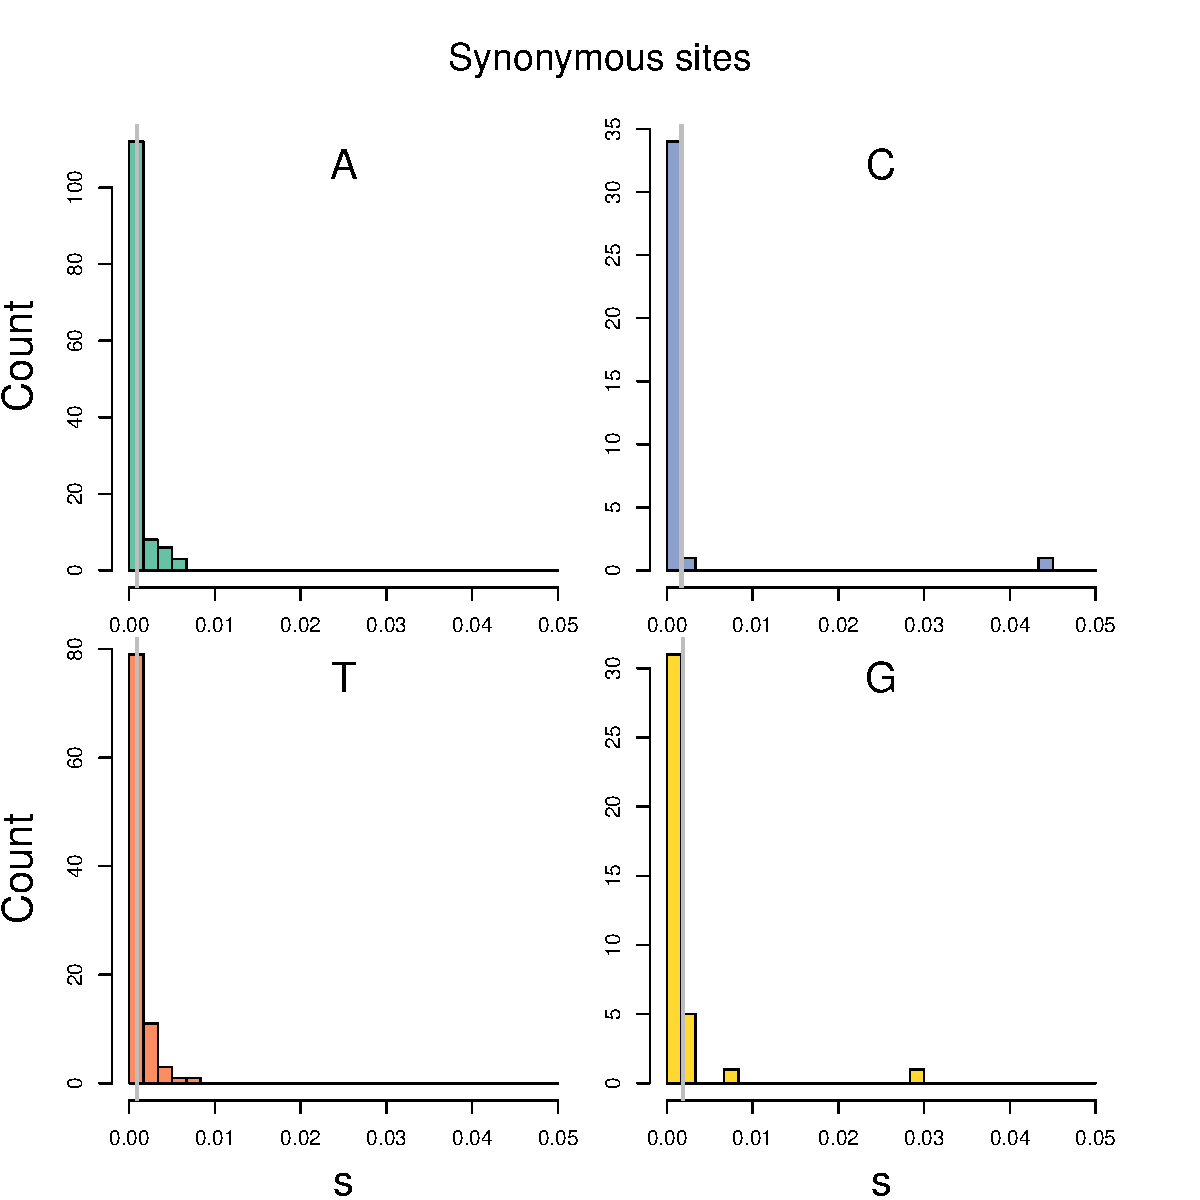
\includegraphics[scale = .45]{F3-Bacheler-syn.pdf}
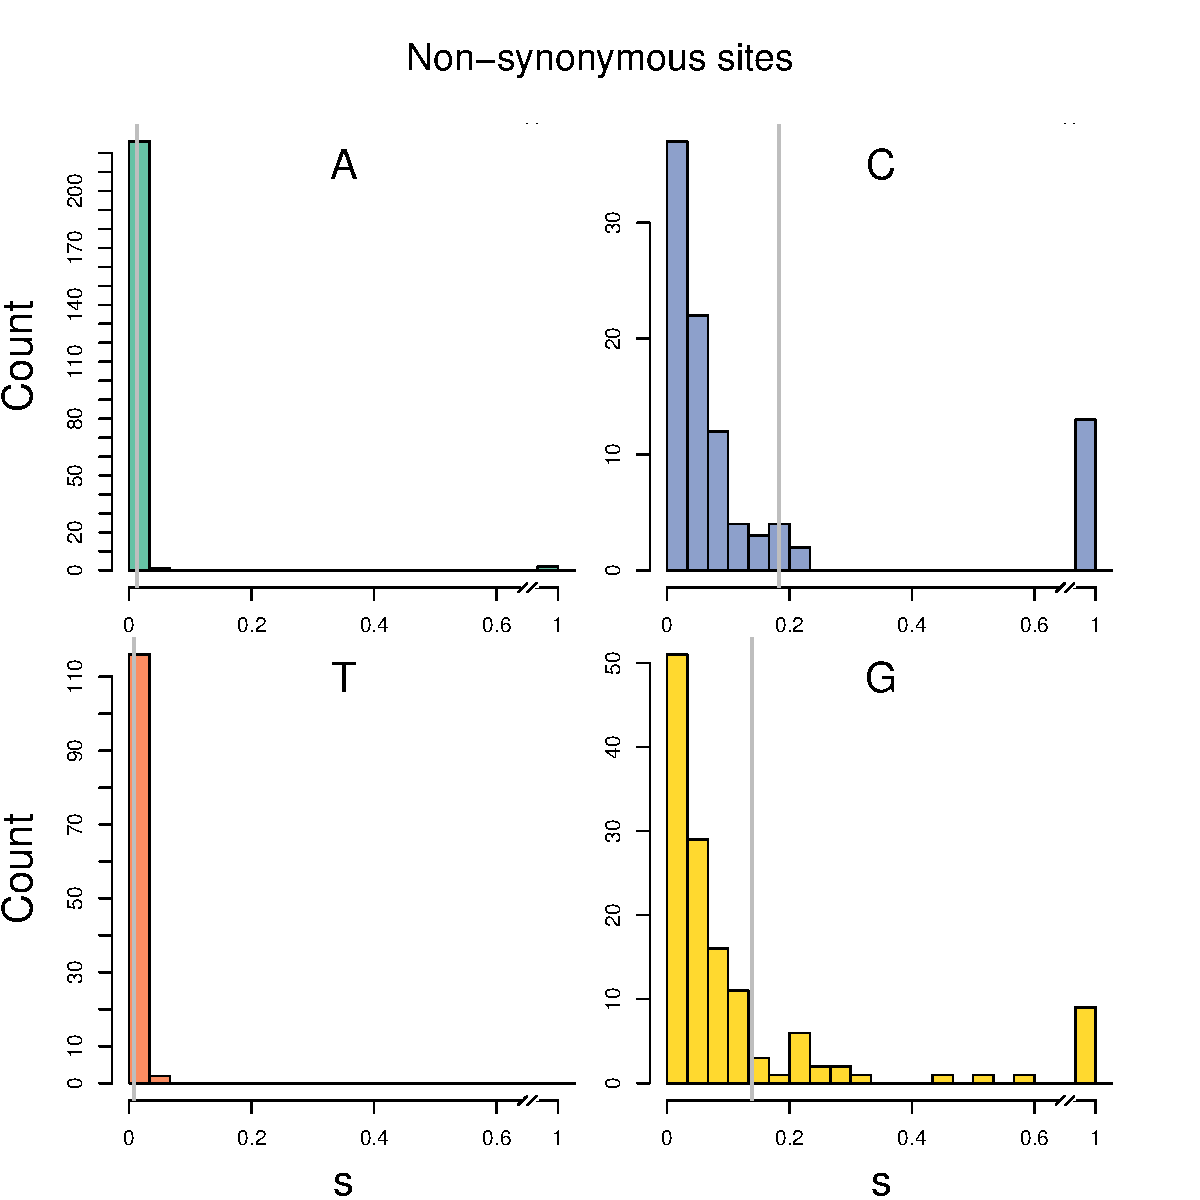
\includegraphics[scale = .45]{F3-Bacheler-nonsyn.pdf}
\caption{Distribution of fitness effects (DFE) for non-synonymous and synonymous mutations \textit {pol}; nonsense mutations are included in the non-synonymous mutations. Note that the scales of the x and y-axis differ between the figures.}
\label{Bachelernonsyn}
\end{figure}

 %\pagebreak
 % Adi: Ok, this is a little confusing. We barely referred to Zanini and Lehman datasets till now, and now they are part of an essential main table. I think this should also be moved to supplementary data...
 % PSP I took out the Zanini and lehman results. We should put them in suppl mats. 
 
\begin{table}[ht!]
\centering
\begin{tabular}{rc|cc|cc|c}
  \hline
  & & Mut. rates from  & Abrahm 2010 & Mut. rates from & Zanini 2016& \\
 & Sites & $\kappa$  & $\theta$ & $\kappa$ & $\theta$ & Lethal \\ 
  \hline
Bacheler & 870 & 0.317 & 0.209 & 0.319 & 0.242 & 0.065 \\ 
    &  & (0.241, 0.397) & (0.202, 0.219) & (0.247, 0.395) & (0.233, 0.253) & (0.05, 0.083) \\ 
  Zanini & 903 & 0.056 & 0.447 & 0.146 & 0.414 & 0 \\ 
     &  & (0.05, 0.061) & (0.421, 0.481) & (0.129, 0.163) & (0.388, 0.443) & (0, 0) \\ 
 Lehman & 540 & 0.155 & 0.238 & 0.228 & 0.258 & 0.013 \\ 
     &  & (0.101, 0.221) & (0.22, 0.261) & (0.169, 0.297) & (0.242, 0.277) & (0.007, 0.021) \\ 
   \hline
\end{tabular}
\label{TableGamma}
\caption{Table with Gamma distribution parameters reflecting scale ($\kappa$) and shape ($\theta$).}
\end{table}

\pagebreak

\subsubsection*{Relationship between within-patient mutation frequencies and site conservation at population level}
We were interested to determine how well the observed within-patient frequencies correspond with world wide frequencies. All sequences from the Bacheler dataset belong to the HIV-1 B subtype, so as a comparison, we collected sequences from the Stanford HIV Drug Resistance database (HIVdb) that were also HIV-1 subtype B. Notably, each such sequence represents the consensus sequence present in a patient (i.e., the consensus of the "mutant cloud" evolving in a patient at a given time point).  HIV subtype B sequences from treatment-naive patients were retrieved from the Stanford Drug Resistance database (HIVdb), with 23742 Protease sequences and 22785 Reverse Transcriptase sequences \cite{rhee2003human}. 
Figure \ref{StanfordVSBacheler} shows the correlation between average within-patient mutation frequencies calculated from the Bacheler dataset and  between-patient mutation frequencies calculated from the HIVdb dataset. A high correlation coefficient was detected when comparing all 870 sites ($R^2= 0.949$), with a higher coefficient for non-synonymous mutations ($R^2 = 0.973$) than for synonymous mutations ($R^2 = 0.884$). In the lower frequency regions, it can be seen that costly mutations occurring at low frequencies within patients are often not observed in consensus sequences of patients. 

\begin{figure}[ht!]
\centering
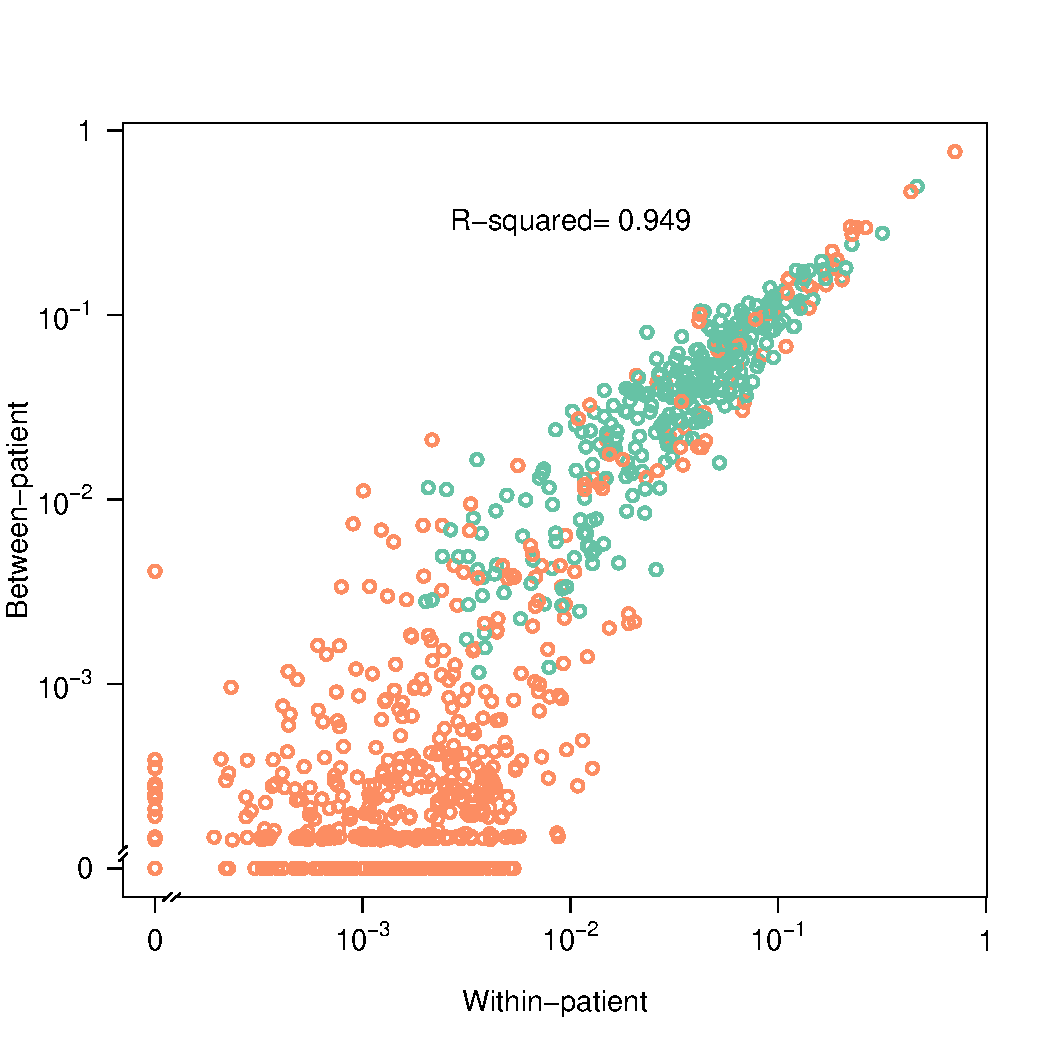
\includegraphics[scale = .65]{F5eLife.pdf}
\caption{Correlation of average mutations frequencies at within-patient level (Bacheler data) and mutation frequencies at between-patient level (HIVdb), with values shown on a log scale. Non-synonymous mutations are shown in red, synonymous mutations are shown in green. }
\label{StanfordVSBacheler} 
\end{figure}


\pagebreak

\section{Conclusion / Discussion}
We used within-patient mutation frequencies for 870 transition mutations in the \textit {pol} gene of HIV as observed in samples from 160 patients \cite{bacheler2000human} to estimate the costs of these mutations for the virus as it evolves in a patient. Due to the high mutation rate of HIV and the large size of our dataset, $93.5\%$ of 870 possible transition mutations were observed in at least one patient in our dataset. Only $6.5\%$ of the mutations (57 mutations) were never observed, but half of these are nonsense mutations that create premature stop codons, so these mutations are expected to be lethal and be swiftly removed due to purifying selection. The other mutations that were never observed may also be lethal, or they may be very costly. A larger dataset would be needed to distinguish between lethal and strongly deleterious mutations. 
We found that the cost of a mutation depends on whether the mutation leads to an amino-acid change, whether that change is drastic or not and whether the mutation creates a new CpG site or not. We also found that G $\rightarrow$ A and C $\rightarrow$ T mutations are generally more costly than A $\rightarrow$ G and T $\rightarrow$ C mutations. 
Other characteristics of sites had smaller effects on the estimated fitness costs, such as the SHAPE parameter which is related to RNA secondary structure (lower SHAPE parameter is associated with a higher cost), and whether a site is part of Protease or Reverse Transcriptase. Our results show that within-patient frequencies of mutations carry a wealth of information on costs of mutations.

\subsubsection*{Comparison with other studies in viruses.}
Our main results are consistent with results from the recent study by Zanini \textit {et al} \cite{zanini2016population}, in that we also find a clear difference between synonymous and non-synonymous mutations (see Supplementary figure \ref{orderedZanini}). One clear difference between the data from our study (based on the Bacheler dataset) and the data from Zanini \textit {et al} is that there are some transition mutations that were never observed in the Bacheler dataset ($6.5\%$ of the sites), whereas all transition mutations were observed in the Zanini dataset. 
A mutation that is not observed will have an estimated fitness cost of $1$, which means that the mutation is lethal. The Bacheler dataset therefore suggests that $6.5\%$ of the mutations are lethal, but the Zanini dataset -if all frequencies are taken at face value - suggests that no mutations are lethal (see Table \ref{TableGamma}). The difference between the two datasets may be due to sequencing depth and sequencing technique. 
In fact, Zanini {\it et al} \cite{zanini2016vivo} filter out mutations that occur at a frequency less than $0.002$, after which roughly $50\%$ of all non-synonymous mutations no longer occur in the  dataset and are therefore considered lethal.  
We didn't do such filtering, but some of the mutations that were not observed in the Bacheler dataset, may have been missed because the sequencing was not very deep (median of 19 sequences per patient). If this is true, then $6.5\%$ is an overestimate. On the other hand, some of the mutations that were observed may be due to sequencing or other errors. 
%For example, nonsense mutations were observed at various frequencies in the Zanini dataset see Supplementary figure \ref{orderedZanini}), even though they are probably lethal and we should observe them at very low frequencies (equal to the mutation rate) or not at all. 
All next-generation sequencing techniques have error rates that are higher than the HIV mutation rates, so the observed frequencies for such mutations are likely overestimates of the real frequencies. The zero percentage of lethal mutations in the Zanini datset is therefore likely an underestimate. 

We also analyzed a third dataset from a recent paper by Lehman {\it et al} \cite{lehman2015risk}\ref{orderedLehman}. In this dataset $1.3\%$ of the transition mutations are never observed and thus estimated to be lethal. Because of the sequencing technology and the associated error rate, we expect that this percentage is also an underestimate of the true percentage of lethal mutations.

It should be noted that even the highest number we found ($6.5\%$ of mutations lethal) is low compared to percentages from \textit {in vitro} studies on coding sequences in viruses (see \cite{sanjuan2010mutational} for an overview). 
For example, Sanjuan {\it et al} \cite{sanjuan2004distribution} find that $40\%$ of random mutations in the RNA virus VSV (Vesicular stomatitis virus) are lethal. 
Another study which used the Tobacco Etch Virus estimated that 27 mutations out of 66 were lethal ($41\%$) \cite{carrasco2007distribution}.
A study by Rihn 
\textit {et al} on the capsid of HIV found that $70\%$ of non-synonymous mutations were lethal, which corresponds to around $47\%$ of all mutations \cite{rihn2013extreme}. 
Two studies on bacteriophage found somewhat lower percentages. Domingo \textit {et al.} found that $20$ or $29\%$ of mutations were lethal (depending on the species) \cite{domingo2009fitness} and Peris \textit {et al.} found that $21\%$ of mutations were lethal \cite{peris2010distribution}.  
% KT : 20 and 29%, what does it mean? PSP: two different species
A recent study on Poliovirus estimated that around $26\%$ of all mutations were lethal \cite{acevedo2014mutational}.
A small study on Phage $\Phi$X174 by Vale \textit {et al.} \cite{vale2012distribution} found that only 1 or 3 out of 36 mutations ($3-8\%$) were lethal which is in the same range as our finding. A few small studies on non-coding regions also found lower percentages of lethal mutations. 
A study on fitness effects in HIV (\cite{van2006effects}) found no lethal mutations out of 15 mutations and a study on a non-coding region in Tobacco Etch Virus found that 2 out of 20 mutations were lethal ($10\%$) \cite{bernet2015distribution}. 

Several factors could contribute to why we find a lower percentage of lethal mutations than \textit {in vitro} studies.
First, we only looked at transition mutations, and excluded transversions from our analysis, but transversions may be more likely to be lethal since they are more often non-synonymous, more often lead to drastic amino acid changes and more often create premature stop codons, due to the nature of the genetic code. 
Second, sequencing, cloning or recording errors may obscure our results. Many low frequency variants in our dataset were only observed once, and it is possible that some of these are not true variants, we may thus underestimate the percentage of lethal mutations. Third, we looked only at one gene, and this gene may have a different fitness landscape than other parts of viral genomes. Finally, it may be that the different environments (\textit {in vitro} vs \textit {in vivo}) or the different genetic backgrounds (usually one genetic background in the \textit {in vitro} studies vs many in \textit {in vivo} studies) lead to the observed differences. We expect that future studies with more sequences and more sites will have better power to determine the true proportion of lethal mutations in HIV \textit {in vivo}. 

\subsubsection*{Factors associated with high fitness costs: nucleotide, amino acid and CpG effect.}

Some of our results are surprising. 
As can be seen in Figure \ref{modeled_sels}, G $\rightarrow$ A mutations appear to be two-and-a-halve to three-and-a-halve times more costly than A $\rightarrow$ G or T $\rightarrow$ C mutations. C $\rightarrow$ T mutations appear to be more costly if they are non-synonymous (six times more costly than A $\rightarrow$ G mutations), but not when they are synonymous. 
It is difficult to determine what causes this nucleotide identity effect. 
First of all, we realize that the effect could be an artifact caused by spurious mutation rate estimates. However, mutation rate estimates from two very different studies Abram {\it et al} \cite{abram2010nature} or Zanini {\it et al} \cite{zanini2016vivo} are very similar and using one or the other does not change our main results. 
Secondly, the nucleotide effect we find may be related to the activity of APOBEC3 enzymes which hypermutate the HIV genome, leading to an increased proportion of G $\rightarrow$ A mutations \cite{sheehy2002isolation, chen2008structure, holden2008crystal}. Thus, it is possible that the G $\rightarrow$ A mutations we observe in the \textit{pol} gene occur together with other G $\rightarrow$ A mutations at other regions in the genome (that we do not observe), leading to a higher fitness cost. 
Third, we hypothesize that the effect may be related to a strong mutation bias in the HIV genome. G $\rightarrow$ A mutations are three to five times more common than A $\rightarrow$ G mutations \cite{abram2010nature, zanini2016vivo}, which could have led, over evolutionary times, to the well known A bias in the HIV genome \cite{van2013nucleotide, van2014nucleotide}. Specifically, sites at which it doesn't matter for viral fitness whether it carries an A or a G would become A biased over time. The result is that A sites are enriched for (nearly) neutral sites and G sites would be depleted of neutral sites, which could lead to G $\rightarrow$ A mutations being more costly, on average, than A $\rightarrow$ G mutations. 
Finally, the effect we observed may be partly due to the specific amino acids that are involved. As can be seen in figure \ref{AA_effect}, most of the very deleterious mutations are concentrated in just a few specific amino acid changes. Studies on larger parts of the genome, or including transversions in addition to transitions, are needed to disentangle the nucleotide and amino acid effects. 

Another factor we find that greatly affects the cost of a mutation is the formation of CpG sites. Depending on the type of sites, CpG forming mutations are between one-and-a-halve and four times more costly than the equivalent mutation that does not create a CpG site. 
In animal and plant genomes, CpG sites are usually found in  promotor regions and their methylation leads to the silencing of the downstream gene \cite{law2010establishing}. It was hypothesized, that these sites occur rarely in coding regions of because methylated cytosines can randomly deaminate to thymine and cause unwanted mutations \cite{scarano1967heterogeneity}. The same mechanism is unlikely to affect a retrovirus like HIV because in HIV most mutations are introduced during reverse transcription and not in the DNA stage.
However, CpG sites are only found very rarely in RNA viruses \cite{rima1997dinucleotide} and strongly selected against in a wide range of viral genomes \cite{cheng2013cpg}. 
Several studies have recently suggested that CpG sites may trigger the antiviral cellular response \cite{burns2009genetic, atkinson2014influence}. A potential reason might be that viral transcripts with CpG are more easily detected by the immune system since CpG sites in animals are usually found in promoters and not in the coding region of genes and therefore rarely transcribed \cite{van2012biased}. 
It was further shown in mutational studies that introducing CpG sites in the viral genome strongly decreased the replication rate \cite{burns2009genetic, atkinson2014influence} and hence the virus' fitness.
Corroborating these previous studies, our analysis shows that CpG site formation has deleterious effects on the fitness of HIV \textit {in vivo}.
Given the ever more convincing evidence that CpG site are deleterious for viral genomes, future efforts should be geared towards the discovery of the molecular mechanism of this process which most likely differs from eukaryotic cells.

\subsubsection*{Limitations of our study.}
A limitation of our study is that we only focused on a small part of the HIV genome, namely 870 sites of the \textit {pol} gene, thereby excluding a large part of the viral genome and all drug resistance mutations, which would be of special interest. 
A second limitation of our analysis is that we only focused on transitions and left out transversion mutations. When deeper and more precise data become available, it would be possible to see how results change when transversions are included. For one, we expect that the distribution of fitness effects will shift towards more costly mutations when transversions are included.  
A third limitation is that we assumed one mutation rate for all A $\rightarrow$ G mutations, and one rate for all C $\rightarrow$ T mutations, etc. There is some evidence that mutation rates may be highly variable, which would mean that we cannot trust selection coefficient estimates for individual mutations \cite{geller2016highly}. 

Another limitation of our study is that it is unknown how long the patients in the Bacheler \cite{bacheler2000human} dataset had been infected before samples were taken. This is relevant because it is known that diversity within a host increases with time \cite{shankarappa1999consistent, kouyos2015irreversibility}. The reason is that most patients are infected with one or a very small number of founder viruses and therefore genetic diversity within the host is usually low right after infection. Over time, genetic diversity accumulates and plateaus after several years. At the same time, the viral population diverges from the founder virus. It is therefore reasonable to ask whether we expect our results to differ depending on when samples were taken. 
First of all, early samples tend to have less genetic diversity, therefore they would carry less information. Mutant frequencies are expected to be close to 0 (if the founder virus is WT at a position) or close to 1 (if the founder virus is mutant at the position). If founder viruses are a random sample from the viral population within a host, then the average mutant frequency across many samples from newly infected patients should be the same as the average mutant frequency across many sample from long term infected patients. For example, if the average frequency of a mutant in all patients in the epidemic is $1\%$, then we expect $1\%$ of the founder viruses to be mutant. Out of 100 newly infected patients, we expect 1 sample to have a mutant frequency at $100\%$ and 99 samples at $0\%$, leading to a $1\%$ average frequency among newly infected patients. The variance of such an average frequency, however, is expected to be very high, because each sample has a frequency of either $0\%$ or $100\%$. Thus, if frequencies in founder viruses and within-host frequencies are similar, then using early samples would lead to unbiased estimates of frequencies, but the variance of such estimate may be very high. It would therefore be better to work with samples from later during the infection. 

Secondly, we should keep in mind that founder viruses may not be a random sample from within-host viruses. If a mutation comes with a fairly severe (but not lethal) cost, such that it is observed within patients at a frequency of 1\%, but it cannot establish a new infection, then we’d expect to see a lower mean frequency in newly infected patients as compared to patients that have been infected longer. Samples from patients that were recently infected could thus be more similar to the wildtype than samples from patients that have been infected for a longer time. This scenario is likely if selection at the beginning of an infection is stronger than selection during an ongoing infection. In a future study it may be possible to compare early and late samples to determine whether such an effect exists. We should note, however, that the tight correlation between within-patient frequencies and global frequencies (see figure \ref{StanfordVSBacheler}) suggests that fitness of HIV strains within hosts and at the infection stage are similar. 

\subsubsection*{Future directions.}
In this study, we have used observed frequencies of transition mutations to estimate fitness costs of mutations. 
%The estimated fitness costs for around 800 sites in Pol, allowed us to see the fitness effect of minor and major AA changes, the creation of new CpG sites and the disturbance of RNA folding. 
Our results demonstrate the power of analyzing mutant frequencies from \textit {in vivo} viral populations to study fitness effects of mutations. We realize however, that the observed frequencies (and thus the estimated costs) between the three datasets we considered differed substantially (see Fig. \ref{orderedBacheler}, \ref{orderedLehman}, \ref{orderedZanini})
\cite{bacheler2000human, zanini2016population, lehman2015risk}. Three key differences exist among the the three datasets: (a) sequencing techniques and associated error rates differed, (b) the viral load among the three studies differed (mainly, in the Zanini dataset viral load was relatively low), and (c) the timing of the samples since infection differed (in the Lehman dataset most samples were at a very early stage of infection). These factors will all influence the frequency measurements, and whether a viral population is at mutation selection balance.
To overcome these issues, a controlled study is necessary, at higher resolution, across more samples and across more sites, ideally using samples from untreated patients. This will allow us to get a more fine-grained and precise picture of costs of mutations at individual sites across the entire HIV genome. 

\pagebreak
\section{Methods}

Most of our analysis is done on the Bacheler \textit {et al.} dataset \cite{bacheler2000human}. 
In addition, we repeat parts of our analysis with the Lehman \textit {et al.} dataset \cite{lehman2015risk} and the Zanini \textit {et al.} dataset \cite{zanini2016population}. 
% Add information on the alignment, and length of RT? 
% KT: mention the reference seq used, this is important to know 

\subsubsection*{Description of the data / filtering}
The Bacheler \textit {et al.} data \cite{bacheler2000human} is cloned and Sanger sequenced, leading to a negligible error rate in the sequences. For each patient, all available sequences are compiled, even though they come from different time points. Patients with only a single sequence were excluded from the analysis, leaving us with a median of 19 sequences per patient and in total 160 patients.
Furthermore, sequences with more than one mutation per triplet were removed, in order to clearly assign a mutation as non-synonymous or synonymous. 

The Lehman data samples are 454 sequenced but exhibit a very high error rate in the sequences. The samples where collected early on after infection, but we only included the time point after seroconversion into our analysis. The sequences span around 600 sites in RT. Since the Lehman data \cite{lehman2015risk} also contain HIV subtypes C and A, we only consider sites that are conserved between subtype A, B and C. 

The Zanini data \cite{zanini2016population} samples are Illumina sequenced and contain multiple time points per patient. The sample collection was usually a few months or more apart and can be treated as independent samples. The Zanini data represent the whole HIV genome, but we only consider the regions that overlap with the Bacheler data \cite{bacheler2000human}.
Also the Zanini data \cite{zanini2016population} contain different HIV subtypes (B and C),  and we therefore only consider sites that are conserved between B and C. 

\subsubsection*{Calculation of frequencies}
For all three datasets, we only consider the more common transition mutations (A$\leftrightarrow$G and C$\leftrightarrow$T). For example, for a site that is A in the ancestral state, the frequency of a transition mutation is calculated for each patient (and each time point in the case of the Zanini data \cite{zanini2016population}) as the number of sequences that carry a G divided by the number of sequences that carry a G or an A. These frequencies are then averaged over all patients (and time points in the case of the Zanini data \cite{zanini2016population}).
Sequences with a C or a T are thus not considered if the ancestral state is A. Selection coefficients are estimated by dividing the nucleotide-specific mutation rate by the average frequency, bootstrapping is done over sites (not patients). 
%For the Generalized Linear Model, actual counts are considered as opposed to frequencies. 


\subsubsection*{Generalized Linear Model}
%KT: i m not sure what we exactly model. From the results, i get selection coefficients, but here i m a bit confused.  Looking back at the results, the first 4 sentences of the GLM section make me say: selection_coefficient ~ .
%PSP: No, the statistics is all on frequencies (or really, counts). Hope that is clear now in the results section. 
We fit a binomial generalized linear model to model the state (ancestral or mutant) of each position based on its ancestral nucleotide, its SHAPE value, whether or not the position is in Reverse Transcriptase and the types of changes resulting from a transition at that position. These changes included whether a transition was non-synonymous, changed the amino acid group (i.e., between the positive-charged, negative-charged, uncharged and hydrophobic groups, or to or from the special amino acids 
% PSP Hey, why are there for special amino acids here ... I added Selenocysteine to the Results section now. 
Cysteine, Selenocysteine, Glycine and Proline) or if the transition formed a new CpG site. We also fit interactions between the ancestral nucleotides, whether a transition was non-synonymous, and whether the transition formed a CpG site.  For the Generalized Linear Model, actual counts are considered as opposed to frequencies. Each position in each sequence from each patient was treated as an independent observation.
Using the results from the GLM, we predict mutant frequencies for certain categories of mutations (e.g., synonymous, non-CpG forming  A$\leftrightarrow$G mutations) and then use the mutation-selection formula ($f = u / s$) to predict the costs of these groups of mutations (see \ref{modeled_sels}. The GLM tests whether a mutant of a certain category is more likely to be present than a mutant of another category. We are, however, interested in whether a mutant of a certain category is more costly than a mutant of another category, which cannot be directly tested in the GLM framework. For example, synonymous C$\leftrightarrow$T mutations are more common than synonymous, non-CpG forming A$\leftrightarrow$G mutations (see figure \ref{modeled_freqs}), but this difference can be explained entirely by the higher mutation rate of C$\leftrightarrow$T mutations, so that the estimated selection coefficients are not different (see figure \ref{modeled_sels}). In order to test explicitly whether two categories of mutations that have different mutation rates have different selection coefficients, we use a one-sided two-sample Wilcoxon test (also known as a Mann-Whitney test). 


%Alison
\subsubsection*{Estimating the gamma distribution}
Gamma distributions were estimated separately for each of the three datasets. Transitions that did not appear and resistance mutation sites were not considered when fitting the gamma distribution. The most likely shape and scale parameters for the data were found using the subplex algorithm implemented in nloptr \cite{nloptr}. Bootstrapped confidence intervals were created by resampling the data with replacement and re-estimating the gamma distribution parameters. Selection coefficients estimated using the mutations rates given both in Abram \textit {et al.} \cite{abram2010nature} and Zanini \textit {et al.} \cite{zanini2016vivo}.


%Kristof
\subsubsection*{Comparison with the global epidemic}
%Diversity at the population level subtype B 
A large HIV-1 sequence dataset was retrieved from the Stanford HIV Drug Resistance Database (HIVdb) \cite{rhee2003human}. \textit{Protease} and \textit{reverse transcriptase} sequences were downloaded in separate files. Sequences that met the following criteria were included in the analysis: treatment-naive status of the host, classification as HIV-1 subtype B and a single sequence per host (selected at random). In total 23742 \textit{protease} and 22785 \textit{reverse transcriptase} sequences were collected. Average mutation frequencies for each site were calculated as explained above. The Pearson product-moment correlation coefficient ($R^2$) was used to quantify the within-patient and between-patient frequency correlation. 

\section{Acknowledgements}
Dmitri Petrov, Arbel Harpak, David Enard, Ryan Taylor, Dara Lehman. 

\section{References}

%\singlespacing
\bibliographystyle{ieeetr}
\bibliography{references.bib}

\pagebreak
\section{Supplementary figures}

\begin{figure}[ht!]
\centering
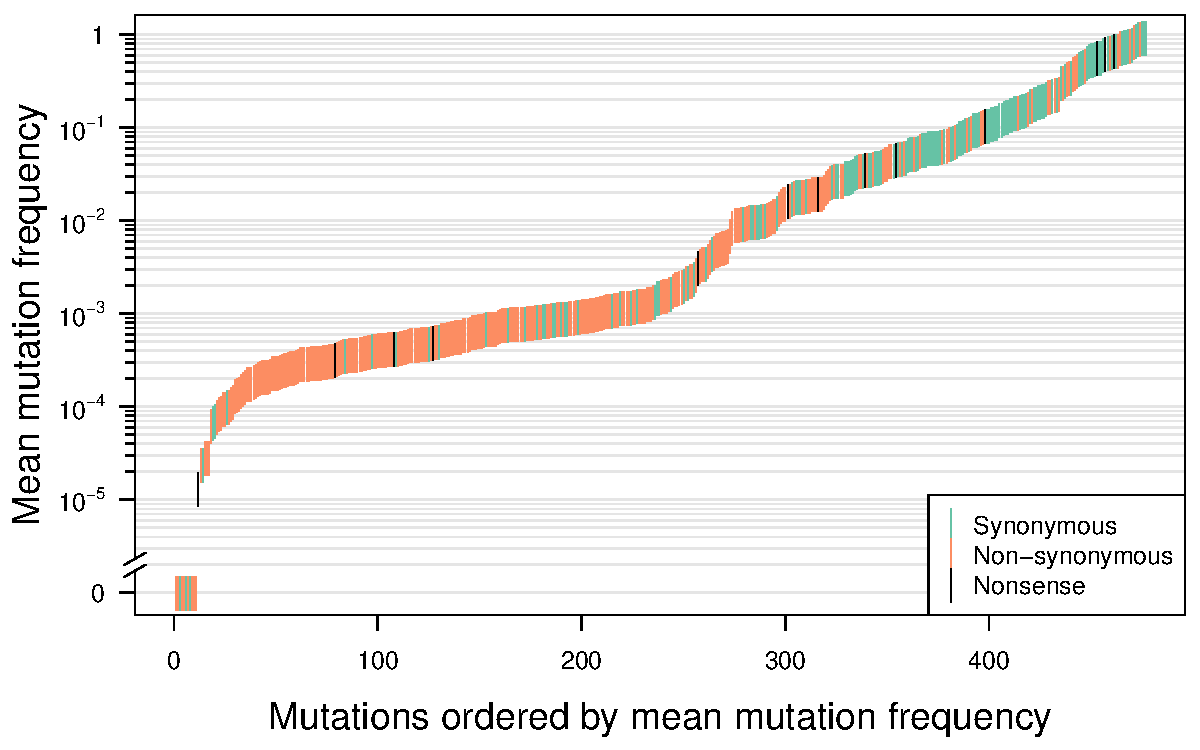
\includegraphics[scale = .7]{F1-ordered-Lehman-cex15.pdf}
\caption{Mutation frequency for 540 sites from the Lehman data, ordered by mutation frequency. Mutations that cause a premature stop codon are shown in black, mutations that cause an amino acid change (non-synonymous) are shown in red and mutations that do not change the amino acid (synonymous) are shown in green.}
\label{orderedLehman}
\end{figure}

\begin{figure}[ht!]
\centering
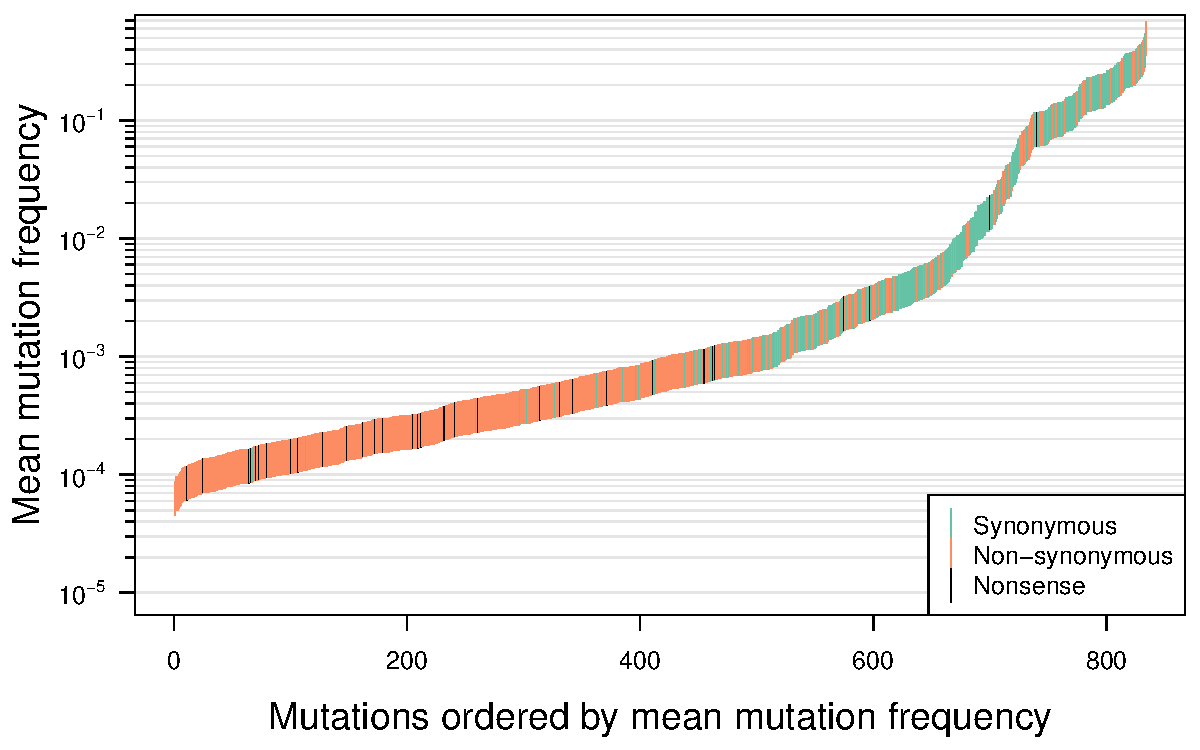
\includegraphics[scale = .7]{F1-ordered-Zanini-cex15.pdf}
\caption{Mutation frequency for 903 pol sites from the Zanini data, ordered by mutation frequency. Nonsense mutations are shown in black, mutations that cause an amino acid change (non-synonymous) are shown in red and mutations that do not change the amino acid (synonymous) are shown in green.}
\label{orderedZanini}
\end{figure}


\begin{figure}[ht!]
\centering
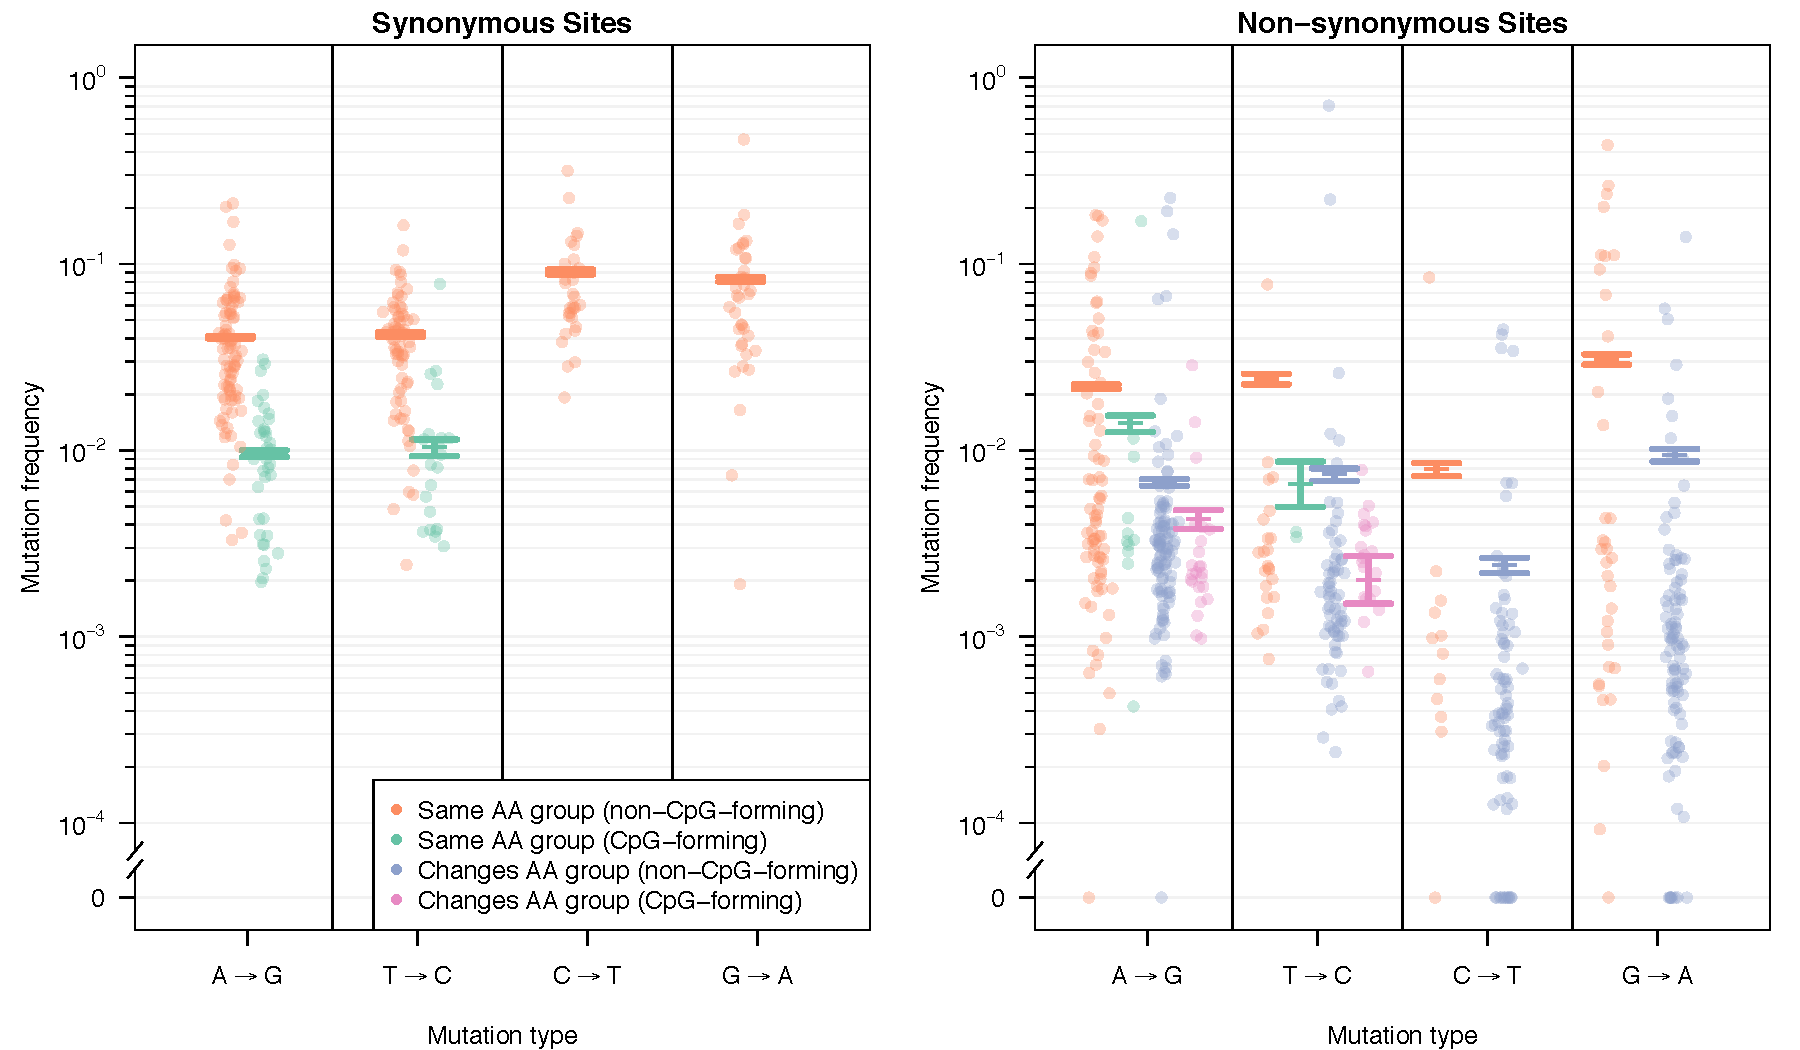
\includegraphics[scale = .55]{modeled_freqs.pdf}
\caption{Generalized Linear Model (GLM) with frequencies estimated from the Bacheler dataset. The graph shows the model predictions for synonymous and non-synonymous mutations that either form CpG sites (green) or do not form CpG sites (orange) by preserving the same amino acid group. For non-synonymous mutations in addition, predictions are shown which change the amino acid group and form CpG sites (pink) or do not form CpG sites (blue). The predictions are shown for the type of nucleotide. The cloud of dots in each panel represents the calculated frequencies found in the Bacheler dataset.}
\label{modeled_freqs}
\end{figure}


\begin{figure}[ht!]
\centering
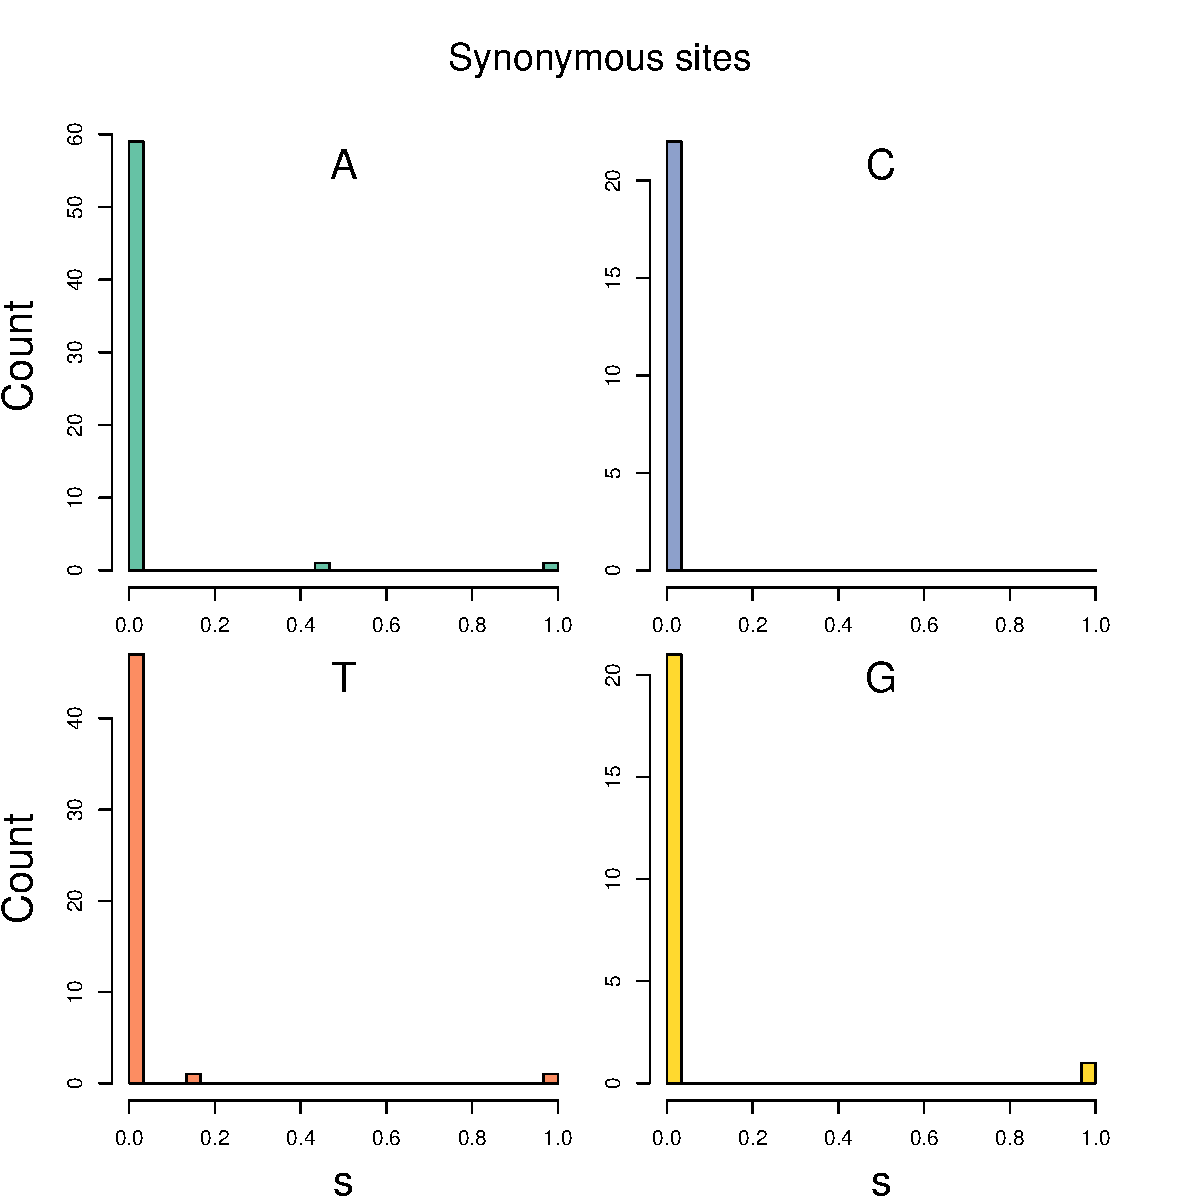
\includegraphics[scale = .45]{F3-Lehman-syn.pdf}
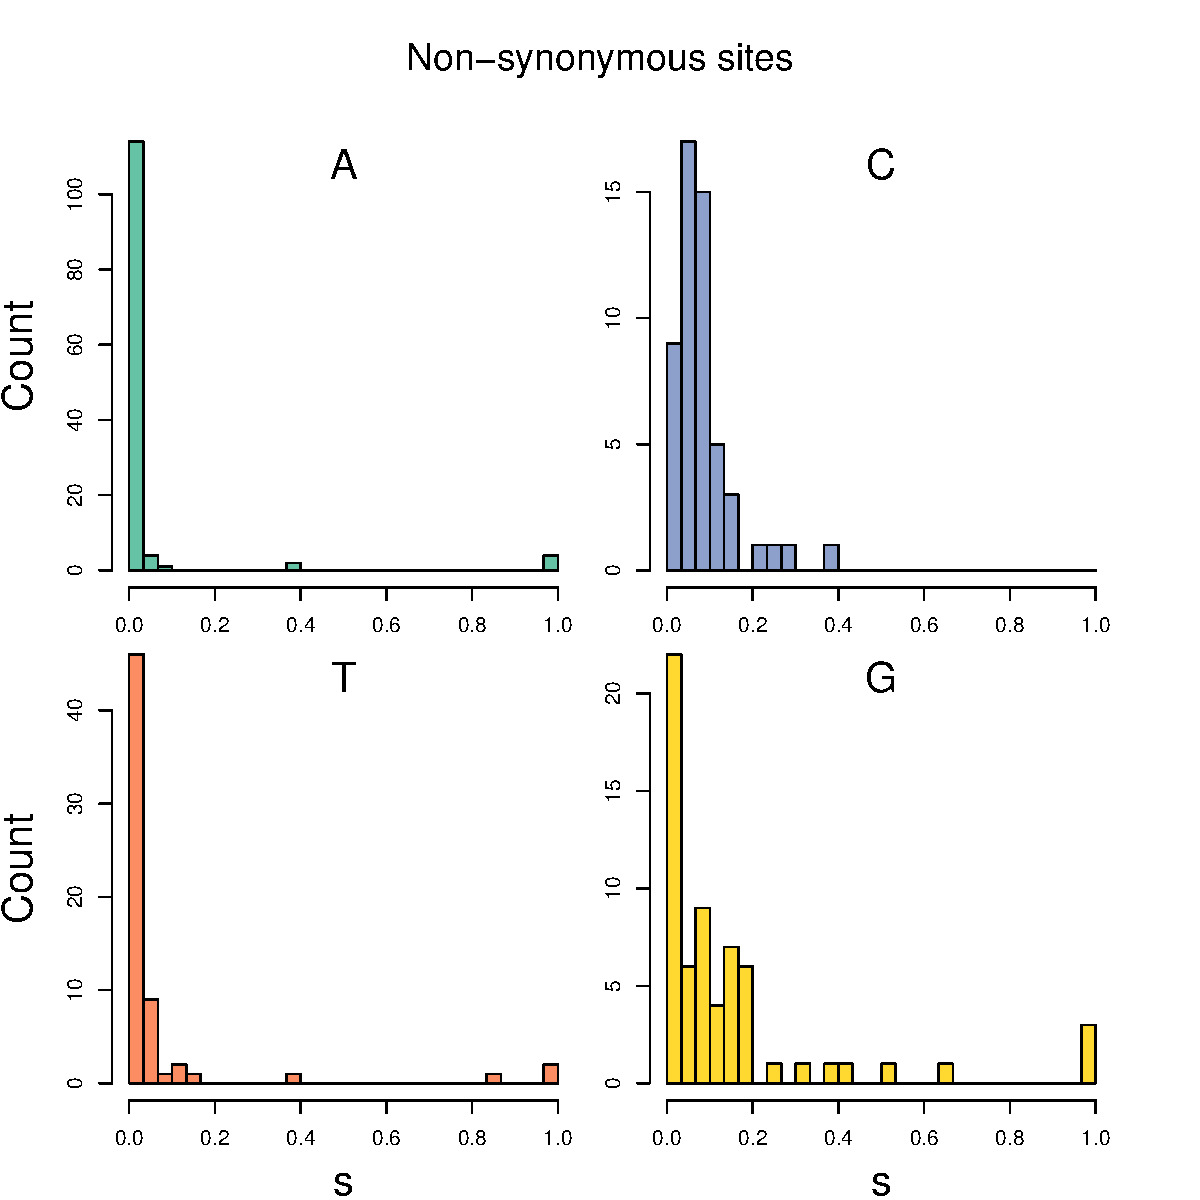
\includegraphics[scale = .45]{F3-Lehman-nonsyn.pdf}
\caption{Distribution of fitness effects (DFE) for non-synonymous and synonymous mutations for the Lehman dataset; nonsense mutations are included in the non-synonymous mutations. Note that the scales of the x and y-axis differ between the figures.}
\label{Lehmannonsyn}
\end{figure}


\begin{figure}[ht!]
\centering
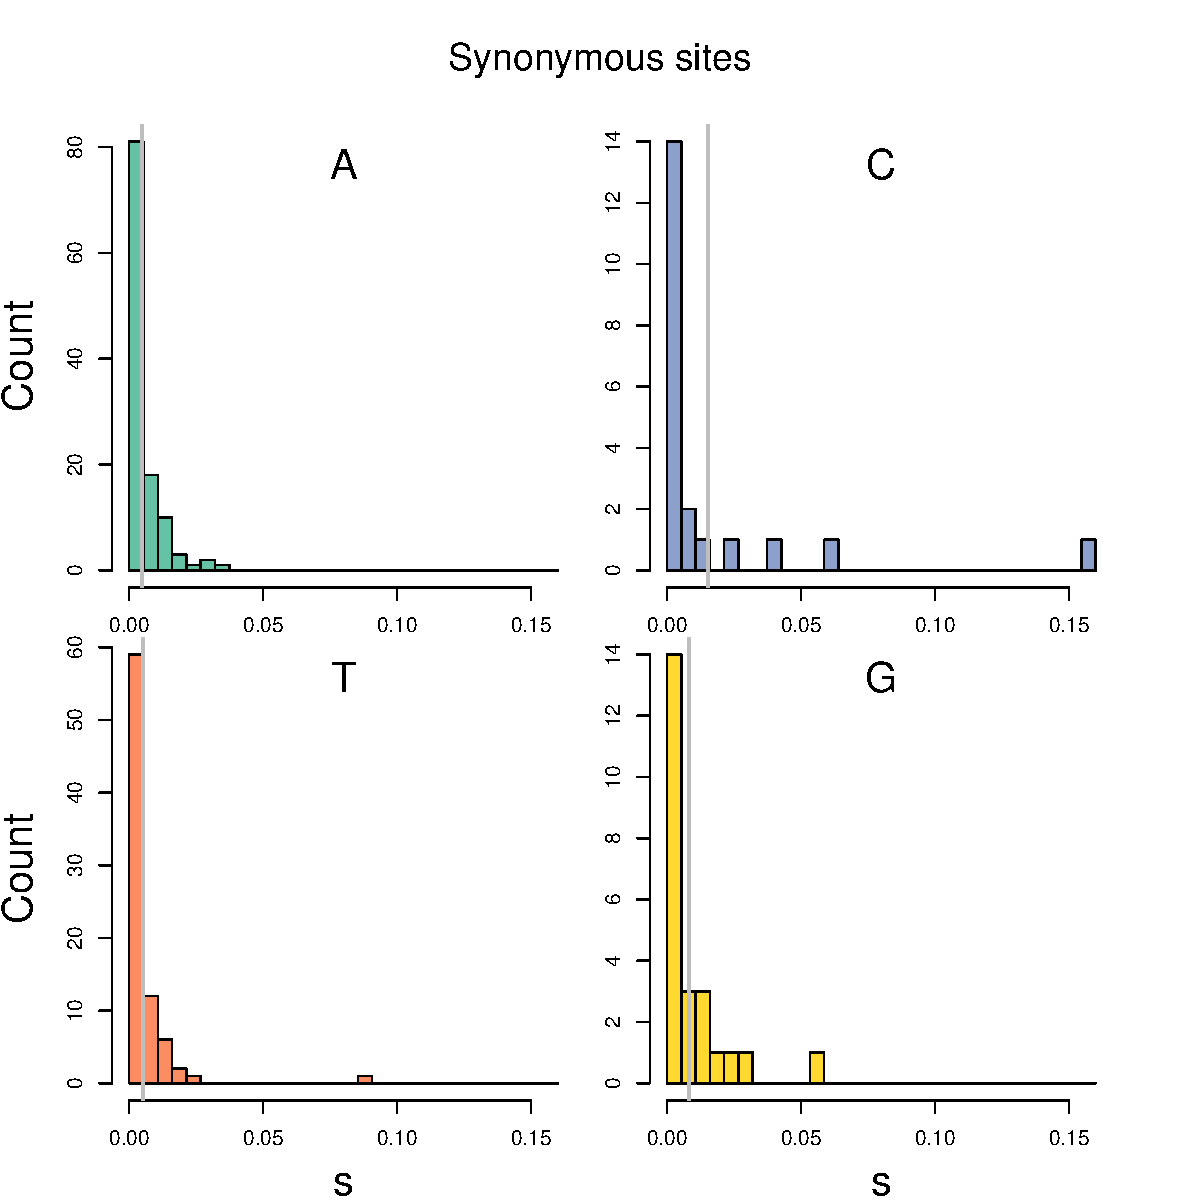
\includegraphics[scale = .45]{F3-Zanini-syn.pdf}
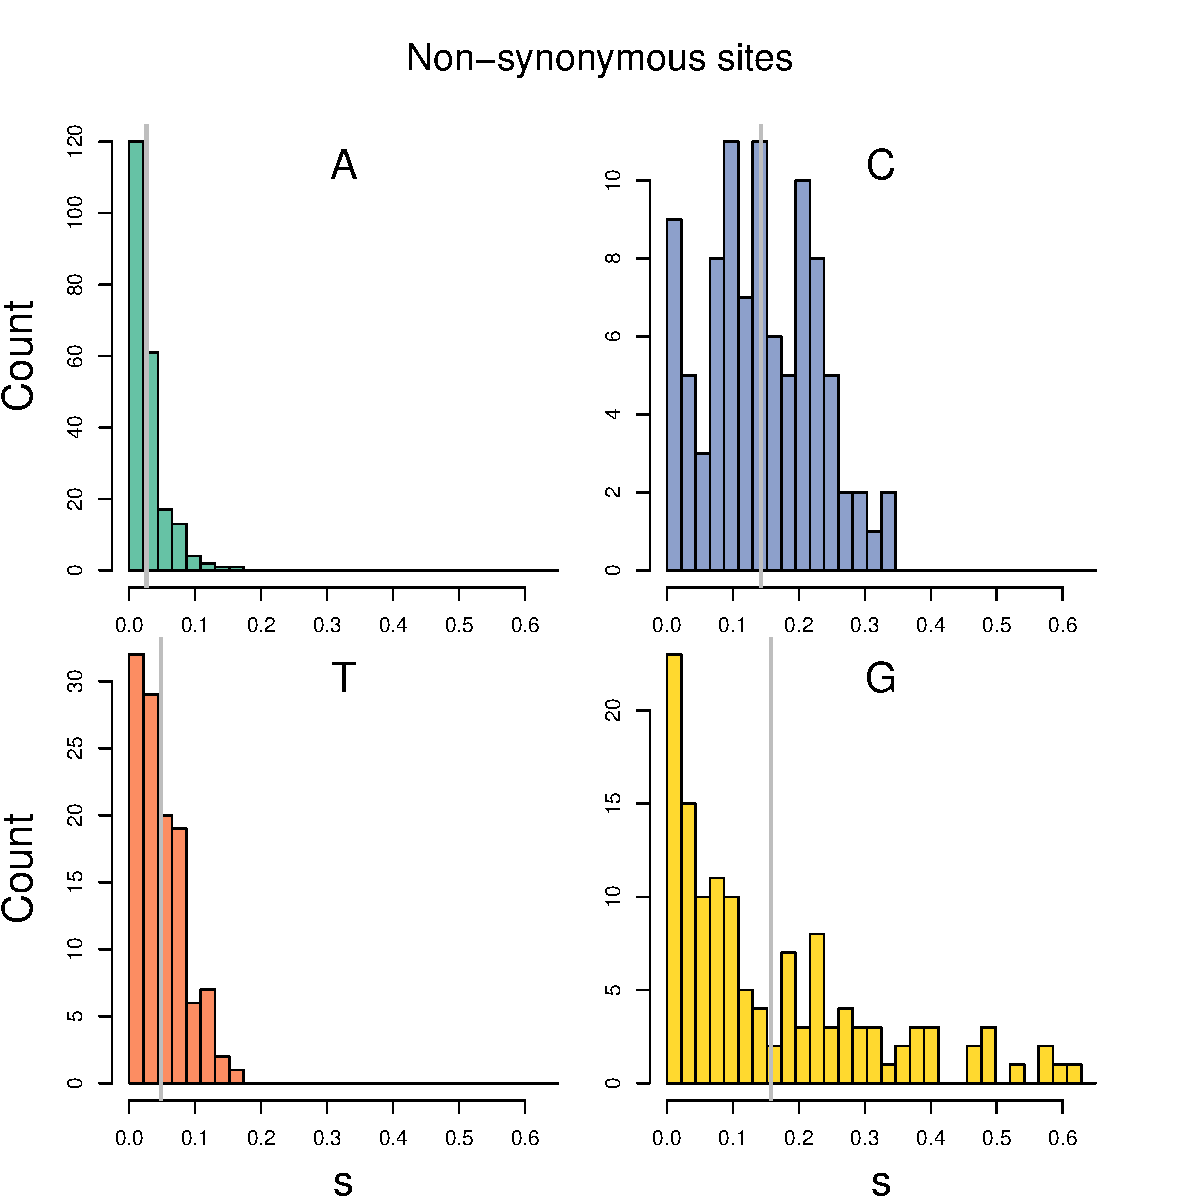
\includegraphics[scale = .45]{F3-Zanini-nonsyn.pdf}
\caption{Distribution of fitness effects (DFE) for non-synonymous and synonymous mutations for the Zanini dataset; nonsense mutations are included in the non-synonymous mutations. Note that the scales of the x and y-axis differ between the figures.}
\label{Zanininonsyn}
\end{figure}

\begin{table}[ht!]
\centering
\begin{tabular}{rc|cc|cc|c}
  \hline
  & & Mut. rates from  & Abrahm 2010 & Mut. rates from & Zanini 2016& \\
 & Sites & $\kappa$  & $\theta$ & $\kappa$ & $\theta$ & Lethal \\ 
  \hline
Bacheler & 870 & 0.317 & 0.209 & 0.319 & 0.242 & 0.065 \\ 
    &  & (0.241, 0.397) & (0.202, 0.219) & (0.247, 0.395) & (0.233, 0.253) & (0.05, 0.083) \\ 
  Zanini & 903 & 0.056 & 0.447 & 0.146 & 0.414 & 0 \\ 
     &  & (0.05, 0.061) & (0.421, 0.481) & (0.129, 0.163) & (0.388, 0.443) & (0, 0) \\ 
  Lehman & 540 & 0.155 & 0.238 & 0.228 & 0.258 & 0.013 \\ 
      &  & (0.101, 0.221) & (0.22, 0.261) & (0.169, 0.297) & (0.242, 0.277) & (0.007, 0.021) \\ 
   \hline
\end{tabular}
\label{TableGammaSupp}
\caption{Table with Gamma distribution parameters reflecting scale ($\kappa$) and shape ($\theta$) for Bacheler, Zanini and Lehman datasets.}
\end{table}


\end{document}

%Section for eLife submission only
%\section{Figures and Tables}

%ordered frequencies
%\begin{figure}[ht!]
%\centering
%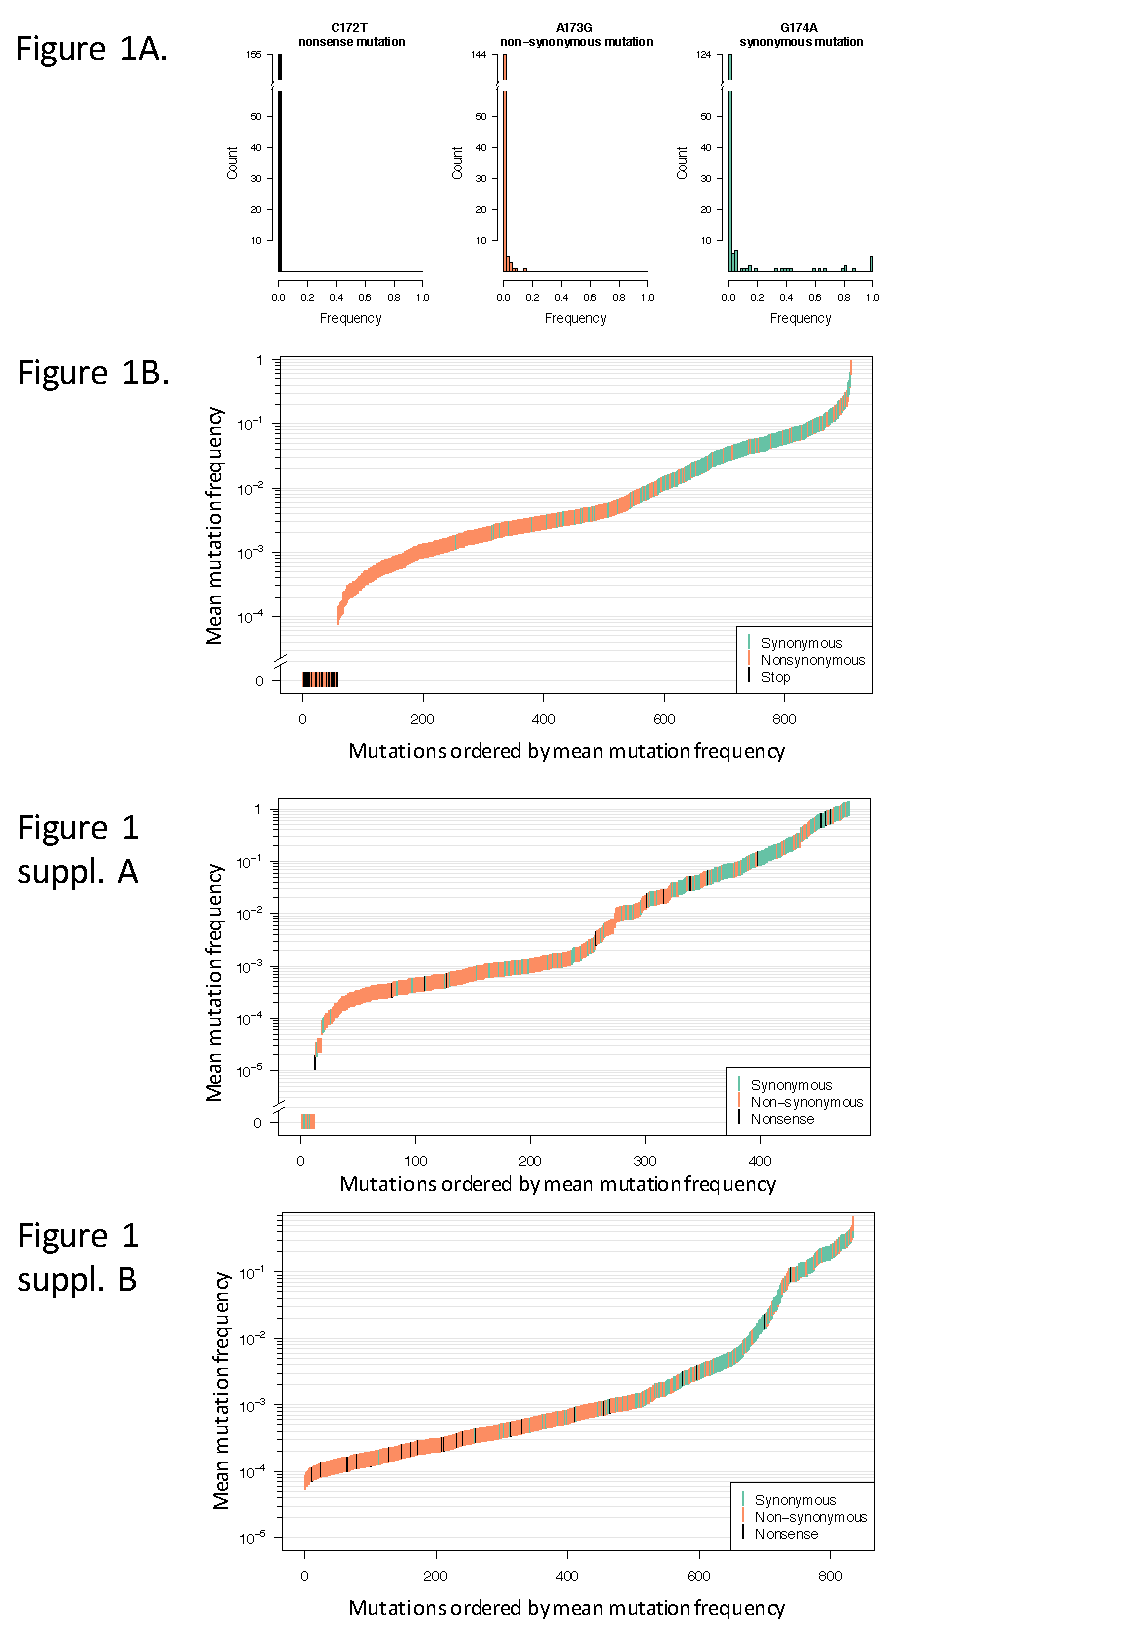
\includegraphics[scale = .8]{F1eLife.pdf}
%\caption{1A.The distribution of mutation frequencies plotted for single sites in the Protease protein (site 172 = nonsense mutation,  site 173 = non-synonymous mutation, site 174 = synonymous mutation). 1B) Mean mutation frequencies for all sites of the Bacheler dataset are shown ordered by mutation frequency. Nonsense mutations are shown in black, mutations that cause an amino-acid change (non-synonymous) are shown in red and mutations that do not change the amino-acid (synonymous) are shown in green.
%S1A.Mutation frequency for 540 sites from the Lehman data, ordered by mutation frequency. 
%S1B.Mutation frequency for 903 pol sites from the Zanini data, ordered by mutation frequency. 
%}
%\label{F1}
%\end{figure}



%GLM selection coefficient and frequencies
%EDIT caption!!!
%\begin{figure}[ht!]
%\centering
%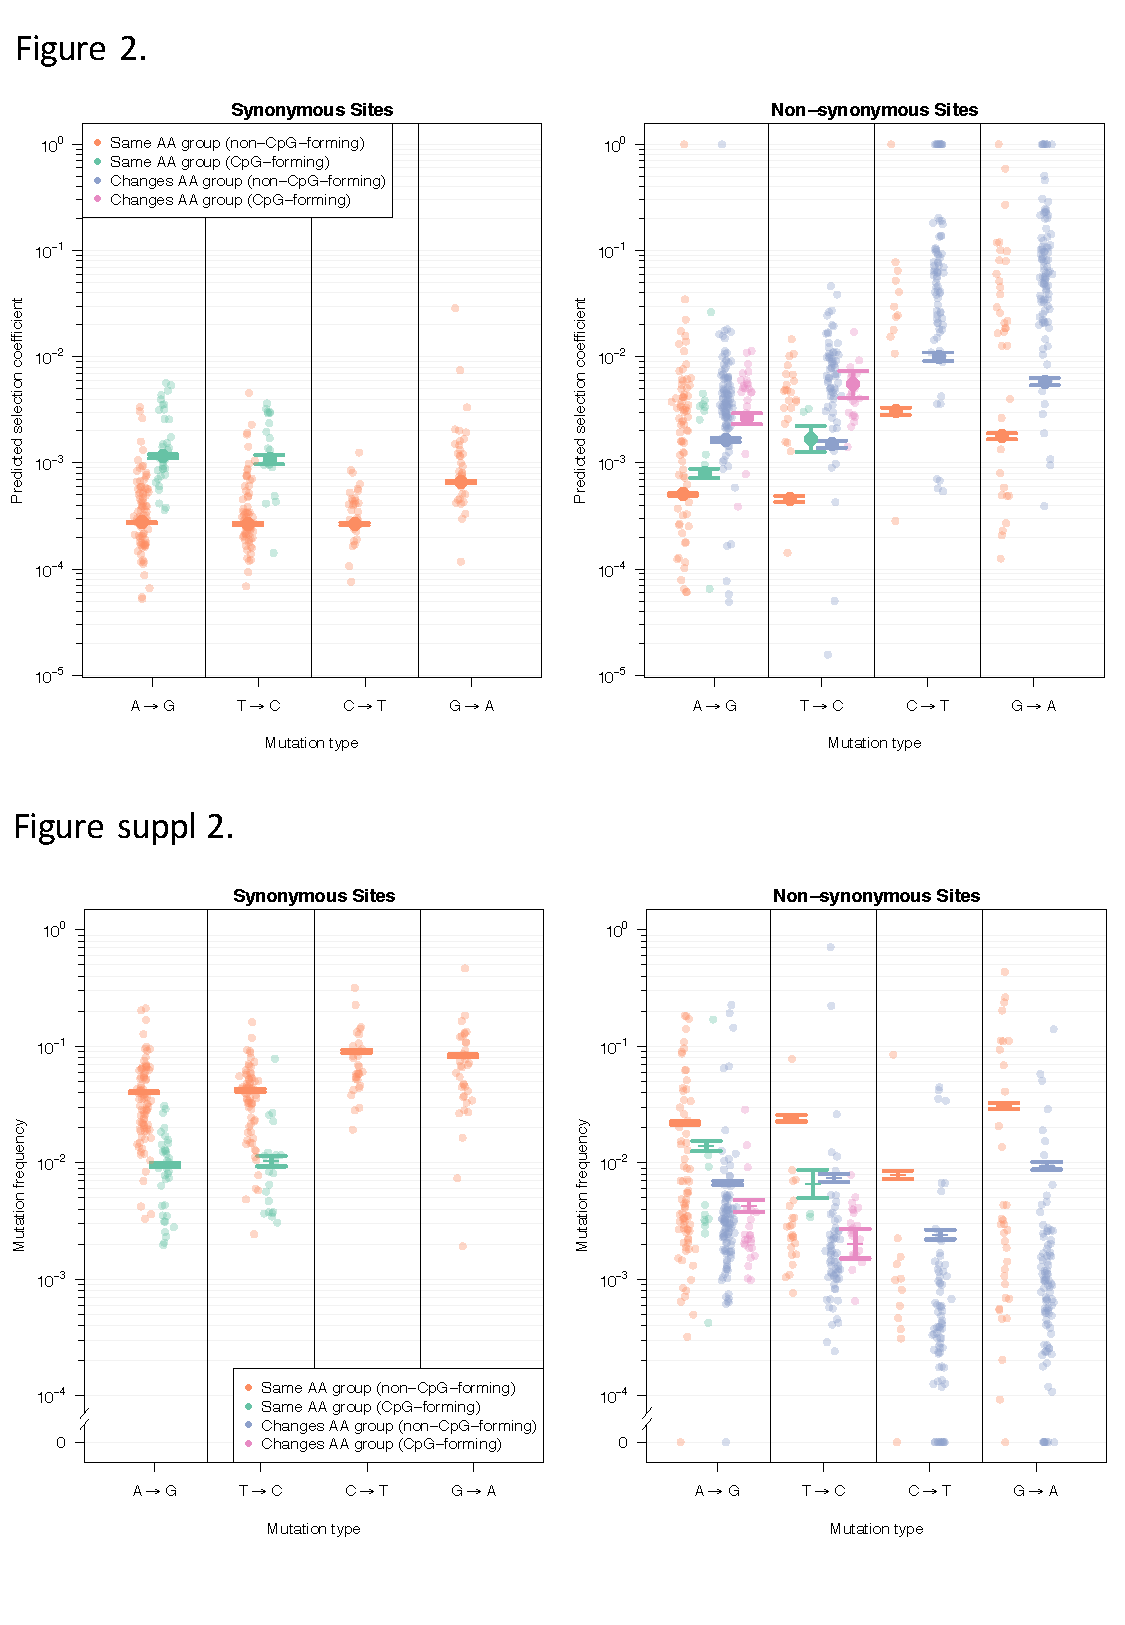
\includegraphics[scale = .8]{F2eLife.pdf}
%\caption{Generalized Linear Model (GLM) with selection coefficients estimated from the Bacheler dataset. The graph shows the model predictions for synonymous and non-synonymous mutations that either form CpG sites (green) or do not form CpG sites (orange) by preserving the same amino acid group. For non-synonymous mutations in addition, predictions are shown which change the amino acid group and form CpG sites (pink) or do not form CpG sites (blue). The prediction are shown for every single nucleotide. The cloud of dots in each panel represents the estimated selection coefficients found in the dataset.
%S2.Generalized Linear Model (GLM) with frequencies estimated from the Bacheler dataset. }
%\label{F2}
%\end{figure}

%\pagebreak

%AA change
%\begin{figure}[ht!]
%\centering
%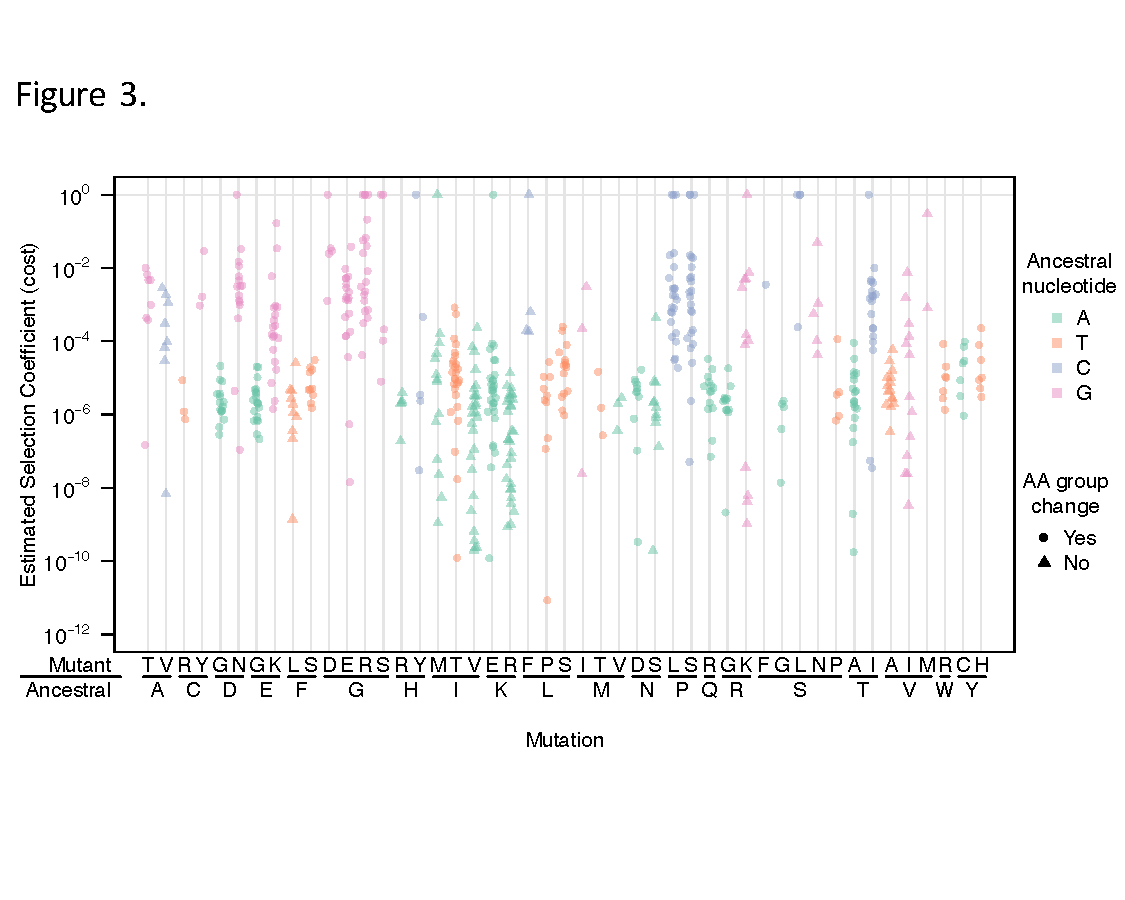
\includegraphics[scale = 1.0]{F3eLife.pdf}
%\caption{Estimated costs of non-synonymous mutations, ordered by ancestral and mutant amino acid. Colors indicate the different nucleotides, shapes indicate whether the AA change is drastic or not.}
%\label{F3}
%\end{figure}

%\pagebreak

%DFE 
%\begin{figure}[ht!]
%\centering
%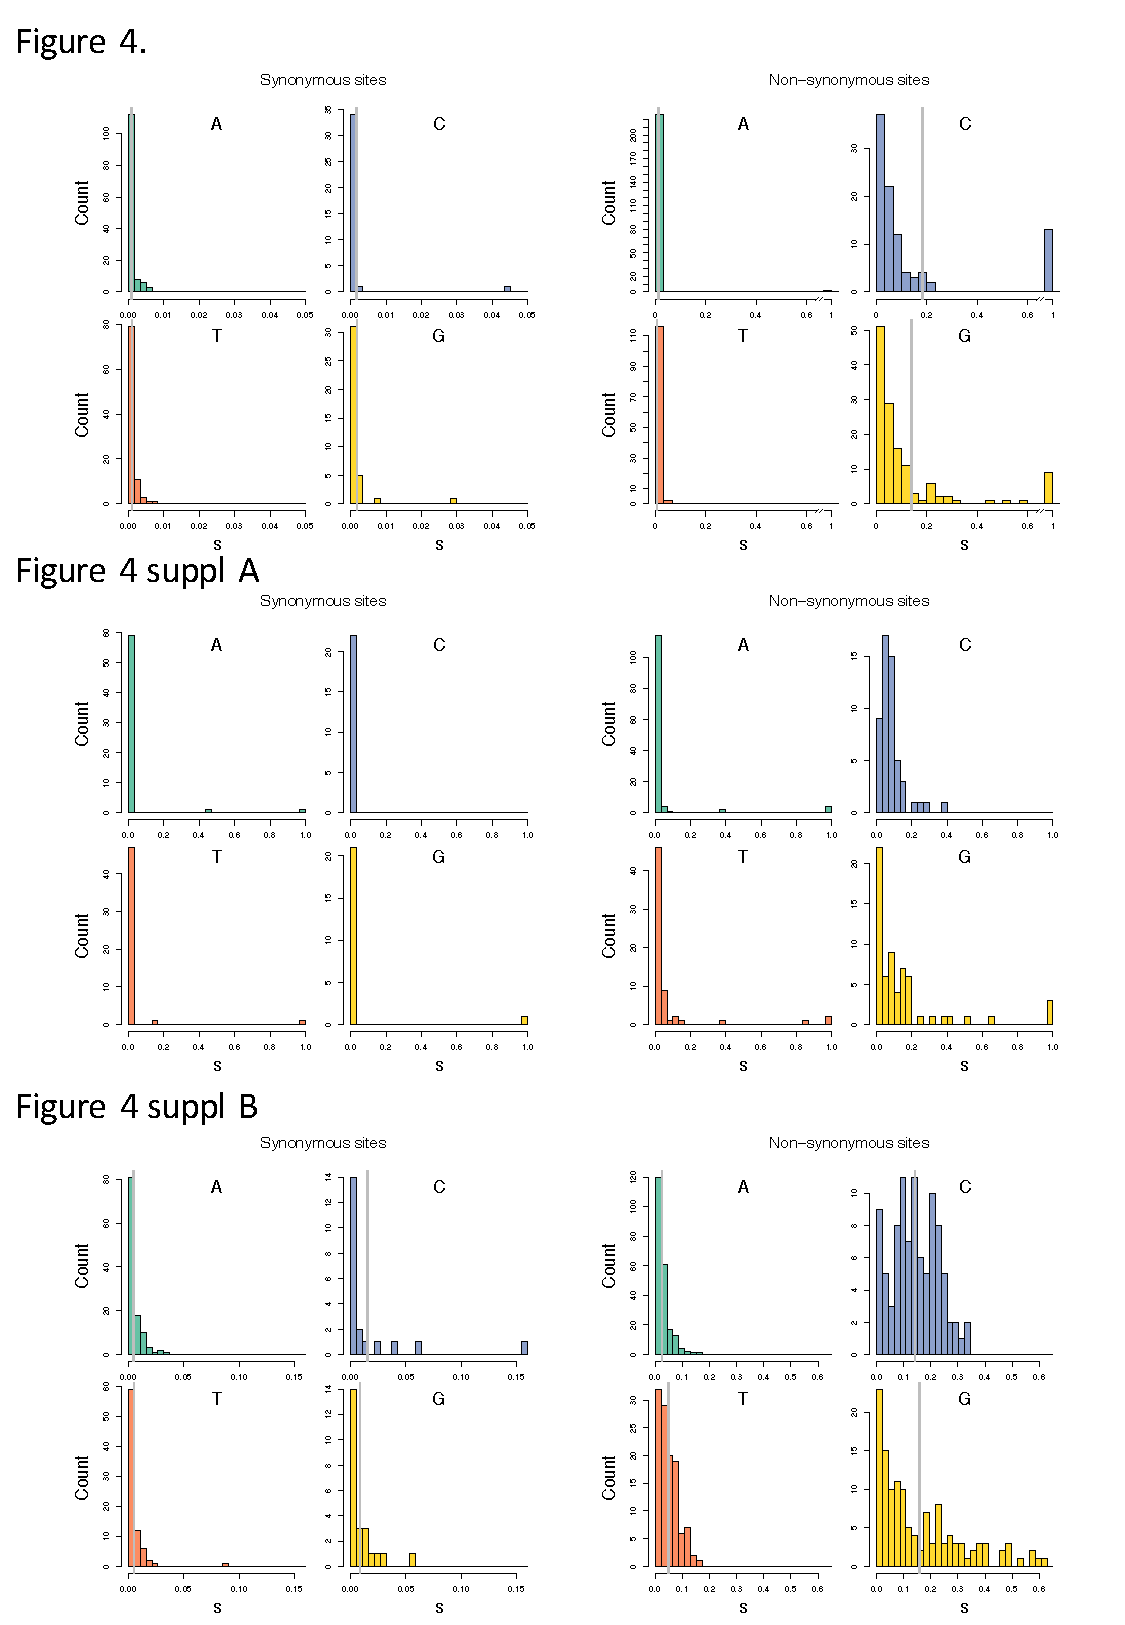
\includegraphics[scale = .8]{F4eLife.pdf}
%\caption{Distribution of fitness effects (DFE) for synonymous and non-synonymous mutations in the Bacheler dataset; nonsense mutations are included in the non-synonymous mutations. Note that the scales of the x and y-axis differ between the figures.
%S4A. Distribution of fitness effects (DFE) for synonymous and non-synonymous mutations in the Lehman dataset.
%S4B. Distribution of fitness effects (DFE) for synonymous and non-synonymous mutations in the Zanini dataset.}
%\label{F4}
%\end{figure}

%\pagebreak

%StanfordVsBacheler
%\begin{figure}[ht!]
%\centering
%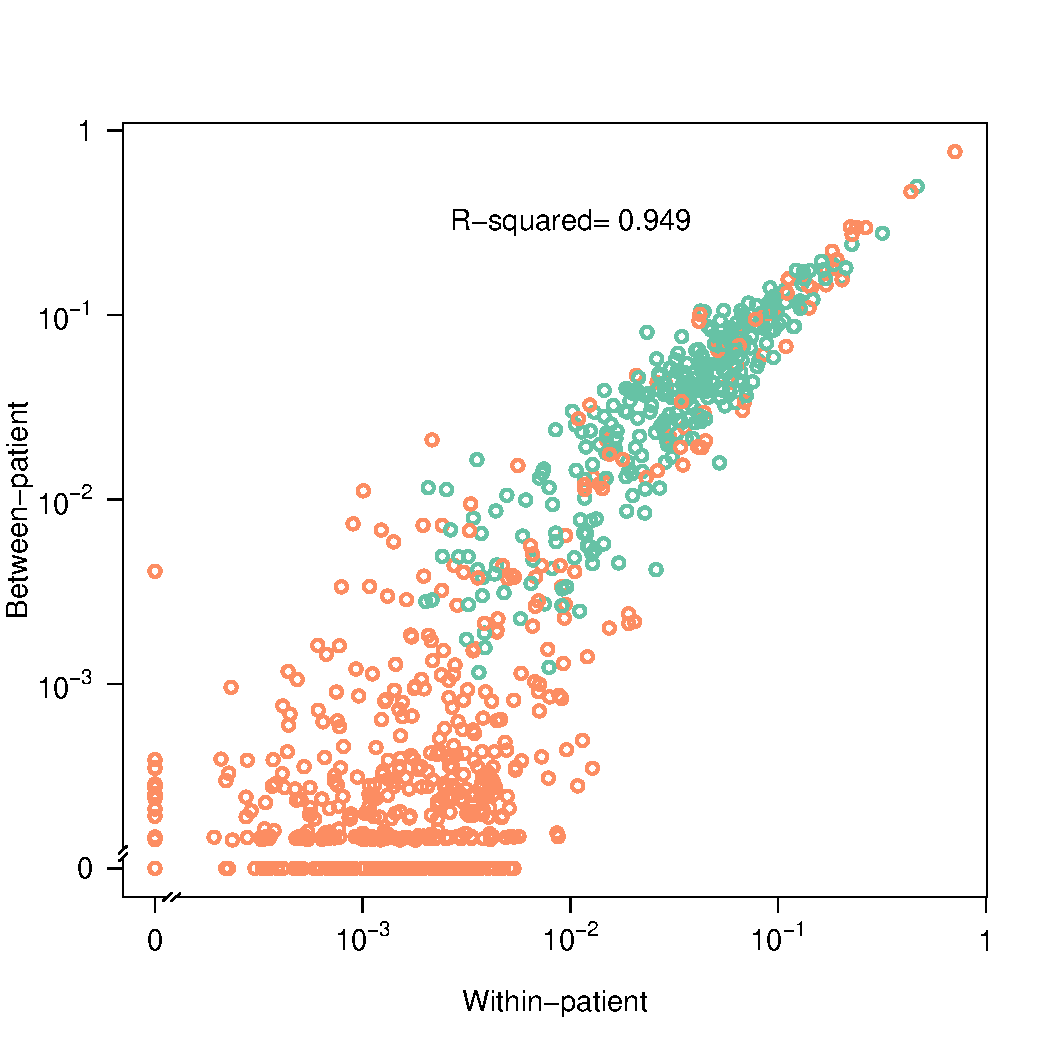
\includegraphics[scale = .65]{F5eLife.pdf}
%\caption{Correlation of average mutations frequencies at within-patient level (Bacheler data) and mutation frequencies at the between-patient level (HIVdb), with values shown on a log scale. Non-synonymous mutations are shown in red, synonymous mutations are shown in green. }
%\label{StanfordVSBacheler} 
%\end{figure}


%Tables for eLife submission
%Table GLM results
%\begin{table}[ht!]
%\centering
%\begin{tabular}{lrrrr}
%  \hline
% & Estimate & Std. Error & z value & Pr($>$$|$z$|$) \\ 
%  \hline
%(Intercept) & -3.208 & 0.013 & -244.671 & 0.000 \\ 
% inRT & 0.136 & 0.008 & 16.206 & 0.000 \\ 
%  shape & 0.169 & 0.014 & 12.034 & 0.000 \\ 
%  \hline
%  t & 0.034 & 0.014 & 2.422 & 0.015 \\ 
%  c & 0.808 & 0.016 & 50.379 & 0.000 \\ 
%  g & 0.717 & 0.014 & 49.936 & 0.000 \\ 
%   CpG & -1.439 & 0.029 & -49.853 & 0.000 \\ 
%   t:CpG & 0.041 & 0.047 & 0.875 & 0.381 \\ 
%   \hline
%  nonsyn & -0.611 & 0.014 & -42.644 & 0.000 \\ 
%  t:nonsyn & 0.061 & 0.024 & 2.551 & 0.011 \\ 
%  c:nonsyn & -1.833 & 0.037 & -49.396 & 0.000 \\ 
%  g:nonsyn & -0.380 & 0.021 & -18.065 & 0.000 \\ 
%  nonsyn:CpG & 0.981 & 0.045 & 21.991 & 0.000 \\ 
%  t:nonsyn:CpG & -0.881 & 0.093 & -9.447 & 0.000 \\ 
%  bigAAChange & -1.183 & 0.014 & -83.501 & 0.000 \\ 
%\hline

%   \hline
%\end{tabular}
%\caption{Table with GLM results for observed counts of mutants. Significant predictors are listed together with their associated P-value based on a Z-test.}
%\label{GLM_results}
%\end{table}



% Table Gamma distribution
%\begin{table}[ht!]
%\centering
%\begin{tabular}{rc|cc|cc|c}
%  \hline
%  & & Mut. rates from  & Abrahm 2010 & Mut. rates from & Zanini 2016& \\
% & Sites & $\kappa$  & $\theta$ & $\kappa$ & $\theta$ & Lethal \\ 
%  \hline
%Bacheler & 870 & 0.317 & 0.209 & 0.319 & 0.242 & 0.065 \\ 
%    &  & (0.241, 0.397) & (0.202, 0.219) & (0.247, 0.395) & (0.233, 0.253) & (0.05, 0.083) \\ 
%  Zanini & 903 & 0.056 & 0.447 & 0.146 & 0.414 & 0 \\ 
%     &  & (0.05, 0.061) & (0.421, 0.481) & (0.129, 0.163) & (0.388, 0.443) & (0, 0) \\ 
%  Lehman & 540 & 0.155 & 0.238 & 0.228 & 0.258 & 0.013 \\ 
%      &  & (0.101, 0.221) & (0.22, 0.261) & (0.169, 0.297) & (0.242, 0.277) & (0.007, 0.021) \\ 
%   \hline
%\end{tabular}
%\label{TableGamma}
%\caption{Table with Gamma distribution parameters reflecting scale ($\kappa$) and shape ($\theta$) for Bacheler, Zanini and Lehman datasets.}
%\end{table}


%%%%%%%%%%%%%%%%%%%%%%%%%%%%%%%%%%%%%%%%%%%%%%%%%%%%%%%%%%%%%%%%%%%%%%%%%%%%%%%%%%%%%%%%%%%%%%%%%%%%%%%%%%%%%%%%%%%%%%%

% latex table generated in R 3.2.3 by xtable 1.8-2 package
% Tue Mar 29 14:21:28 2016
%\begin{table}[ht]
%\centering
%\begin{tabular}{rc|cc|cc|c}
%  \hline
%  & & Abrahm 2010 & & Zanini 2016 & & \\
% & Sites & Scale & Shape & Scale & Shape & Lethal \\ 
%  \hline
%Bacheler & 984 & 0.317 & 0.209 & 0.319 & 0.242 & 0.065 \\ 
%    &  & (0.241, 0.397) & (0.202, 0.219) & (0.247, 0.395) & (0.233, 0.253) & (0.05, 0.083) \\ 
%  Zanini & 903 & 0.056 & 0.447 & 0.146 & 0.414 & 0 \\ 
%     &  & (0.05, 0.061) & (0.421, 0.481) & (0.129, 0.163) & (0.388, 0.443) & (0, 0) \\ 
%  Lehman & 540 & 0.155 & 0.238 & 0.228 & 0.258 & 0.013 \\ 
%      &  & (0.101, 0.221) & (0.22, 0.261) & (0.169, 0.297) & (0.242, 0.277) & (0.007, 0.021) \\ 
%   \hline
%\end{tabular}
%\end{table}

% latex table generated in R 3.2.3 by xtable 1.8-2 package
% Wed Apr 13 16:08:37 2016
%\begin{table}[ht]
%\centering
%\begin{tabular}{lrrrr}
%  \hline
% & Estimate & Std. Error & z value & Pr($>$$|$z$|$) \\ 
%  \hline
%(Intercept) & -3.208 & 0.013 & -244.671 & 0.000 \\ 
% inRT & 0.136 & 0.008 & 16.206 & 0.000 \\ 
%  shape & 0.169 & 0.014 & 12.034 & 0.000 \\ 
%  \hline
%  t & 0.034 & 0.014 & 2.422 & 0.015 \\ 
%  c & 0.808 & 0.016 & 50.379 & 0.000 \\ 
%  g & 0.717 & 0.014 & 49.936 & 0.000 \\ 
%   CpG & -1.439 & 0.029 & -49.853 & 0.000 \\ 
%   t:CpG & 0.041 & 0.047 & 0.875 & 0.381 \\ 
%   \hline
%  nonsyn & -0.611 & 0.014 & -42.644 & 0.000 \\ 
%  t:nonsyn & 0.061 & 0.024 & 2.551 & 0.011 \\ 
%  c:nonsyn & -1.833 & 0.037 & -49.396 & 0.000 \\ 
%  g:nonsyn & -0.380 & 0.021 & -18.065 & 0.000 \\ 
%  nonsyn:CpG & 0.981 & 0.045 & 21.991 & 0.000 \\ 
%  t:nonsyn:CpG & -0.881 & 0.093 & -9.447 & 0.000 \\ 
%  bigAAChange & -1.183 & 0.014 & -83.501 & 0.000 \\ 
%\hline



%   \hline
%\end{tabular}
%\end{table}

%Old table version
% latex table generated in R 3.2.3 by xtable 1.8-2 package
% Wed Mar 30 16:28:40 2016
%\begin{table}[ht]
%\centering
%\begin{tabular}{rrrr}
%  \hline
% & Estimate & Std. Error & Pr($>$$|$z$|$) \\ 
%  \hline
%(Intercept) & -2.99 & 0.01 & 0.00 \\ 
%  t & 0.16 & 0.01 & 0.00 \\ 
%  c & 0.80 & 0.02 & 0.00 \\ 
%  g & 0.85 & 0.01 & 0.00 \\ 
%  bigAAChange & -1.22 & 0.01 & 0.00 \\ 
%  inRT & 0.14 & 0.01 & 0.00 \\ 
%  nonsyn & -0.48 & 0.01 & 0.00 \\ 
%  shape & 0.13 & 0.01 & 0.00 \\ 
%  CpG & -1.16 & 0.02 & 0.00 \\ 
%  pairingprob & -0.78 & 0.01 & 0.00 \\ 
%  t:nonsyn & 0.03 & 0.02 & 0.27 \\ 
%  c:nonsyn & -1.94 & 0.04 & 0.00 \\ 
%  g:nonsyn & -0.54 & 0.02 & 0.00 \\ 
%   \hline
%\end{tabular}
%\end{table}
%

\end{document}


AF/MG: How exactly are the resistance mutations called? PSP I went off of Johnson 2010 – but it may be good to check the list I have, it's in an ugly R script! 
MH: visualising the error rate of the NGS datasets in the ordered frequency figures would be nice. PSP: Not sure how that should be done. 
MG: taking different mutation rates and see how much it affects our results. PSP: sounds good to me! 
MG: take a look into structural protein elements like a helices and beta barrels. PSP: I'd love to see the reulst from the more complete/ complex GLM. 

